% HealthScore Research Manuscript — LaTeX Project
% Target Publication Format: Springer Lecture Notes in Computer Science (LNCS)
\documentclass[runningheads]{llncs}

\usepackage[T1]{fontenc}
\usepackage{graphicx}
\usepackage{amsmath,amssymb,amsfonts}
\usepackage{booktabs}
\usepackage{tabularx}
\usepackage{url}
\usepackage{color}
\usepackage[hidelinks]{hyperref}
\usepackage{microtype}
\usepackage{array}

% Formatting configuration
\graphicspath{{figures/}}

\begin{document}

\title{Evaluating High-Throughput Permissioned Blockchain for Healthcare Workflows: Fabric Performance with ACG-Inspired Risk Scoring and Premium Simulation}
\titlerunning{Evaluating Permissioned Blockchain for Healthcare Workflows}

\author{Anonymous Author(s)}
\authorrunning{Anonymous Author(s)}

\institute{Anonymous Institution(s)\\
\email{anonymous@institution.org}}

\maketitle

\begin{abstract}
\sloppy
Permissioned distributed ledger architectures hold significant promise for healthcare administration, clinical auditability, and multiparty insurance workflows by providing distributed verification, role-based access control, and tamper-evident state recording. However, enterprise adoption is hindered by uncertainty regarding transaction throughput ceilings, consensus queueing latency under load, and the computational cost of integrating off-chain risk inference with on-chain state recording. Furthermore, resilience under actual peer, orderer, storage, or network failures has not been established by fault-injection experiments.

In this paper, we evaluate \textbf{HealthScore}, an integrated architecture coupling a 5-organization Hyperledger Fabric consortium network (Hospital, Patient, Pharmacy, Diagnostic Laboratory, and Health Insurer) with an off-chain Adjusted Clinical Group (ACG)-inspired multi-disease risk model and an exploratory premium simulation. We establish three distinct, non-overlapping performance evidence streams: (i)~an authoritative historical empirical Hyperledger Caliper benchmark across $24,500$ transactions (commit \texttt{944fb0d}), (ii)~a verified live Caliper rerun on an isolated 5-organization testbed executing the expanded 11-round workload ($31,500$ transactions), and (iii)~a reproducible stochastic fluid-queueing performance model across 100 seeds exploring theoretical saturation dynamics.

Our empirical blockchain benchmarks demonstrate: (1)~\textbf{Sub-100ms Linear Operating Regime:} Across representative synthetic healthcare benchmark workloads (\texttt{createPatientRecord}, \texttt{updateHealthScore}, \texttt{createPrescription}, and \texttt{requestScan}), the Fabric network scales linearly up to $200$ transactions per second (TPS) with committed throughput of $199.9$--$200.2$ TPS, average confirmation latency below $0.06$ seconds ($0.03$--$0.04$s median), and zero reported failures among submitted transactions ($0/24,500$ historical, $0/31,500$ live 11-round). (2)~\textbf{Distinct Saturation and Queueing Regimes:} Under a nominal 1,000 TPS offered load governed by Raft consensus batching, CouchDB endorsement write validation, and block-cutting boundaries (\texttt{BatchTimeout: 2s}, \texttt{MaxMessageCount: 10}), observed throughput and latency vary with client worker concurrency and execution conditions. In the historical baseline, the network saturated at $350.1$ TPS committed write throughput at a $963.6$ TPS send rate ($18.00$s average latency); the 5-worker isolated testbed achieved $515.8$ TPS throughput at a $615.7$ TPS send rate ($6.98$s average latency); and the corrected 8-worker stress repetitions sustained $485.27 \pm 14.60$ TPS ($\text{ddof}=1$; individual runs: $470.6$, $499.8$, $485.4$ TPS) at a $742.70 \pm 62.62$ TPS actual send rate ($5.36 \pm 0.22$s average latency) with zero reported failures among submitted transactions ($0/25,480$). (3)~\textbf{Decoupled Read Scalability:} Local peer CouchDB state evaluation (\texttt{getPatientRecord}) scales linearly across 100, 250, and 500 TPS to $500.3$--$500.6$ TPS by bypassing orderer consensus and multi-peer validation, with displayed average latency $\le 0.01$s (Caliper reports latency to two decimal places; max $0.04$--$0.13$s). (4)~\textbf{End-to-End Application Throughput Boundary:} We explicitly distinguish smart contract chaincode capacity ($350$--$515$ write / $500$ read TPS) from the end-to-end web client pipeline. The HTTP Express API, JWT authorization, and Python machine learning subprocess inference incur execution overhead ($\approx 40$--$50$ ms), bounding a single synchronously awaiting worker process to an estimated $\approx 20$--$25$ requests per second ($1 / 0.045\text{s} \approx 22.2\text{ req/s}$) rather than an observed multi-client stress measurement, confirming that production deployments must decouple inference via asynchronous message queues.

We contextualize this distributed ledger capability with an audited machine learning pipeline evaluated across 46,458 records from three official Medical Expenditure Panel Survey (MEPS) cohorts (HC-251, HC-256, and HC-257 Panel 28 prospective follow-up). Controlled 17-scenario feature ablations show that custom ACG-inspired condition clusters provide the primary predictive improvement over demographic baselines (increasing dollar regression $R^2$ from $0.0395$ to $0.0771$ and doubling weighted Brier Skill Score from $+0.0506$ to $+0.1005$), while composite interaction terms yield modest incremental variance ($\Delta R^2 = +0.0027$) despite dominating tree-based SHAP attribution ($39.0\%$). Our deployment candidate---an 11-feature Observable Logistic Regression (Weighted Fit) targeting survey-weighted P90 high-expenditure risk ($P_{90,\text{wtd}} \ge \$17,827.41$, base prevalence $10.51\%$)---achieves ROC-AUC $0.7654$ [95\% CI: $0.7444$, $0.7881$], PR-AUC $0.3184$ [95\% CI: $0.2876$, $0.3556$], and weighted Brier Skill Score $+0.1025$. Evaluated at a predicted-probability threshold of $\hat{p} \ge 0.10$, it achieves precision of $0.2318$ (an unweighted enrichment of approximately $1.93\times$ over the $11.98\%$ unweighted test prevalence) and recall of $0.7733$ (distinct from selecting a top-10\%-ranked cohort). Disclosed weaknesses include nominal dollar underestimation by log-models, lagged-expenditure baseline dominance ($R^2 = 0.1204$), absence of decision-curve analysis, and the inability to compute standardized Charlson or Elixhauser indices due to unreleased ICD-10 codes. Finally, we formalize a transparent, exploratory Value-at-Risk premium simulation $X_\alpha = B + (1+\alpha)G$ where dimensionless risk-loading $\alpha \ge 0$ scales synthetic Gamma loss above a base-cost floor $B$; empirical simulations across 60 scenarios calibrate to analytical Gamma quantiles within $0.7\%$, though commercial underwriting adequacy remains uncertified.

\keywords{Permissioned Blockchain \and Hyperledger Fabric \and Caliper Benchmarking \and Healthcare Systems \and Risk Adjustment \and Tweedie Regression \and Value-at-Risk.}
\end{abstract}

% -----------------------------------------------------------------------------
\section{Introduction and Research Questions}
% -----------------------------------------------------------------------------
Modern healthcare information systems must simultaneously satisfy rigorous throughput, auditability, and data confidentiality requirements. Clinical care, prescription issuance, diagnostic imaging, and insurance risk adjustment involve multiple distinct legal entities---hospitals, outpatient clinics, retail pharmacies, diagnostic laboratories, and insurance carriers. In traditional centralized architectures, these entities exchange records through point-to-point electronic data interchange (EDI) clearinghouses or centralized payer databases. Such centralized architectures suffer from proprietary data silos, high reconciliation overhead, single points of compromise, and the absence of an immutable, shared audit trail across institutional boundaries.

Permissioned distributed ledger technology (DLT), specifically Hyperledger Fabric~\cite{androulaki2018hyperledger}, offers an enterprise-grade alternative by establishing a shared, append-only, cryptographically verified ledger governed by multi-organization consensus, role-based access control via Membership Service Providers (MSPs), and deterministic smart contracts (chaincode). However, adopting permissioned blockchain in healthcare requires rigorous empirical evidence rather than theoretical assumptions:
\begin{enumerate}
    \item Can a permissioned consortium sustain representative healthcare write transaction rates (patient registration, prescription issuance, score recording) with sub-second confirmation latency under realistic block-formation rules?
    \item At what offered load does the network encounter saturation, and how do consensus-backed state writes compare to read-only queries?
    \item How should computationally demanding analytics---such as chronic-disease risk prediction and insurance expenditure forecasting---be architected to avoid burdening the distributed ledger?
    \item What are the empirical performance boundaries when transitioning from isolated chaincode benchmarks to full end-to-end application services?
\end{enumerate}

Crucially, while permissioned blockchains provide cryptographic auditability and distributed consensus, resilience under actual peer, orderer, storage, or network failures has not been established by fault-injection experiments. Furthermore, comparative privacy evaluation against encrypted databases was outside the study's scope; data confidentiality is evaluated solely via Membership Service Provider authorization policies.

To address these empirical questions, we investigate \textbf{HealthScore}, an audited enterprise architecture that decouples compute-heavy risk modeling and loss simulation into an off-chain engine while anchoring patient milestones, diagnostic requests, prescriptions, and verified risk scores onto an on-chain 5-organization Hyperledger Fabric network. The primary contribution of this work focuses on empirical blockchain throughput, latency, saturation behavior, and the performance boundary between the ledger layer and the end-to-end web client, while machine learning ablations and an exploratory premium simulation serve as supporting contributions.

\subsection{Explicit Research Questions}
Our investigation is guided by four primary research questions:
\begin{itemize}
    \item \textbf{RQ1 (Throughput \& Latency Scaling):} How do transaction throughput and confirmation latency scale as offered load increases for representative healthcare write operations (\texttt{createPatientRecord}, \texttt{updateHealthScore}, \texttt{createPrescription}, \texttt{requestScan}) versus read-only queries on a 5-organization Fabric network under specified testbed conditions?
    \item \textbf{RQ2 (Saturation Dynamics \& Bottlenecks):} What operating region, saturation knee, queueing trade-off, and transaction failure profile characterize the Fabric network under severe stress loads up to $1,000$ TPS, and how does chaincode throughput diverge from end-to-end application throughput?
    \item \textbf{RQ3 (ACG-Inspired Multi-Disease Incremental Value):} What isolated predictive evidence supports custom ACG-inspired chronic-condition clusters versus composite multimorbidity penalties and age-by-comorbidity interaction terms across dollar expenditure regression and high-cost classification on official survey cohorts?
    \item \textbf{RQ4 (Configurable Risk-Loading Simulation):} How do configurable base-cost floors ($B$) and dimensionless risk-loading parameters ($\alpha$) govern the simulated loss distribution ($X_\alpha = B + (1+\alpha)G$), and how accurately do Monte Carlo simulated quantiles calibrate against analytical Gamma Value-at-Risk targets?
\end{itemize}

% -----------------------------------------------------------------------------
\section{Related Work and Research Gap}
% -----------------------------------------------------------------------------

\subsection{Hyperledger Fabric Architecture and Benchmarking in Healthcare}
Hyperledger Fabric~\cite{androulaki2018hyperledger} has emerged as a widely studied permissioned blockchain framework for enterprise consortia due to its modular execute-order-validate transaction lifecycle. Unlike public proof-of-work blockchains constrained to single-digit TPS (e.g., Bitcoin $\approx 7$ TPS, Ethereum $\approx 15$--$30$ TPS), Fabric executes chaincode endorsements in parallel before ordering transactions into blocks via Crash Fault Tolerant (CFT) Raft consensus~\cite{androulaki2018hyperledger}.

Prior healthcare blockchain studies have proposed conceptual frameworks for electronic health records (EHRs) and consent management. However, many published works rely on qualitative proposals or simulated toy networks of 1--2 nodes, lacking standardized, reproducible performance evaluations. Hyperledger Caliper~\cite{caliper2022} provides a standardized Linux Foundation benchmarking framework to measure throughput, latency, and resource consumption under controlled offered rates. In this work, we deploy Caliper v0.5.0 against an authoritative 5-organization Fabric topology, systematically characterizing both linear and saturated regimes. We evaluate representative synthetic benchmark workloads under a single administrative identity (\texttt{HospitalOrgAdmin}) on a single-host virtualized testbed, clearly distinguishing protocol-level capacity from multi-tenant production healthcare traffic.

\subsection{Clinical Risk Adjustment \& Multi-Disease Grouping}
In health economics, risk adjustment models adjust capitation payments and identify high-cost patients. The Johns Hopkins ACG (Adjusted Clinical Groups) system~\cite{weiner1991development}, CMS Hierarchical Condition Categories (CMS-HCC)~\cite{cms2024report}, and Chronic Illness and Disability Payment System (CDPS)~\cite{kronick2000improving} group thousands of ICD-10 diagnosis codes into clinical clusters.

However, existing commercial groupers are proprietary, centralized, and dependent on complete administrative billing claims unavailable in light digital health intakes. While machine learning researchers have attempted to predict healthcare costs using survey datasets such as MEPS~\cite{ahrq_meps_2023}, published models frequently suffer from training-inference feature leakage (relying on unobservable clinical survey questions), failure to evaluate arithmetic dollar calibration, and lack of prospective multi-year testing. Furthermore, de-identified public MEPS data files do not provide granular 4-character and 5-character ICD-10-CM diagnosis codes due to privacy protections, precluding standardized Charlson Comorbidity Index (CCI) or Elixhauser index calculations. We address this gap by establishing an open, ACG-inspired chronic-condition clustering design evaluated across three successive MEPS releases, acknowledging the absence of formal Charlson/Elixhauser comparisons as a data-driven limitation.

\subsection{Actuarial Loss Simulation \& Risk Loading}
In insurance mathematics, healthcare losses exhibit extreme right-skewness, excess zeros, and heavy upper tails. Actuarial pricing utilizes compound Poisson-Gamma (Tweedie) GLMs~\cite{tweedie1984index} and parametric Value-at-Risk (VaR) simulations to estimate required risk margins above expected losses. While prior health tech demonstrations often confuse statistical confidence intervals with loss percentiles or hardcode static premium offsets, we formulate a transparent, parameterized risk-loading formulation with closed-form analytical calibration. We maintain this simulation strictly as an exploratory technical demonstration, disclaiming commercial pricing certification, underwriting adequacy, and reserve solvency.

% -----------------------------------------------------------------------------
\section{HealthScore Architecture and Healthcare Transaction Lifecycle}
% -----------------------------------------------------------------------------
HealthScore establishes a hybrid off-chain/on-chain architecture designed to maximize throughput while guaranteeing auditability. A Node.js API Gateway verifies inbound client requests using server-validated JSON Web Tokens (JWT) and default-deny role-based access control. Computationally intensive machine learning inference and loss simulations are handled entirely by an off-chain Python engine, which loads SHA-256 verified model artifacts. Once computed, verifiable transaction milestones are committed to the 5-organization Hyperledger Fabric network via the Fabric Gateway SDK.

\subsection{What Remains Off-Chain vs. What is Recorded On-Chain}
To preserve patient privacy under HIPAA/GDPR and prevent ledger bloat, raw clinical notes, free-text intake, biometric sensor streams, and high-dimensional model weight files remain strictly \textbf{off-chain}. Comparative privacy evaluation against encrypted database architectures was outside the scope of this study; we evaluate data-management partitioning and smart contract authorization only to the extent supported by the implemented software.

The blockchain ledger records discrete, verifiable state milestones:
\begin{enumerate}
    \item \texttt{createPatientRecord}: Patient registration with baseline demographic identifiers and initial clinical history.
    \item \texttt{updateHealthScore}: Timestamped health risk score (0--100 percentile rank), model-predicted annual dollar expenditure, and simulated target premium, signed by \texttt{HospitalOrgMSP}.
    \item \texttt{createPrescription}: Cryptographically signed medication order with dosage, frequency, and optional off-chain payload hash.
    \item \texttt{dispensePrescription}: Status update executed exclusively by \texttt{PharmacyOrgMSP} recording dispensing timestamp and pharmacist ID. This establishes an auditable multiparty workflow between prescriber and dispenser, but does not constitute a clinically proven drug-abuse prevention system.
    \item \texttt{requestScan} \& \texttt{completeScan}: Diagnostic order lifecycle managed collaboratively between \texttt{HospitalOrgMSP} and \texttt{LabOrgMSP}.
\end{enumerate}

\subsection{Ledger and World-State Distinction}
Hyperledger Fabric maintains a fundamental architectural duality:
\begin{itemize}
    \item \textbf{Append-Only Block Storage:} An immutable, cryptographic SHA-256 hash-chained log of every transaction block. When a patient's risk score is updated annually, the previous score is never overwritten or erased; the complete longitudinal trajectory remains immutably auditable.
    \item \textbf{CouchDB World-State Database:} A document database maintaining the current state snapshot. Key-based reads (\texttt{getPatientRecord}) execute directly against CouchDB on the endorsing peer without traversing ordering or consensus, achieving low-latency query performance ($\le 0.01$s displayed average, maximum $0.04$s historical / $0.13$s live).
\end{itemize}

\noindent\textit{Fault-Tolerance Disclosure:} Although Raft consensus is Crash Fault Tolerant (CFT) in theory, resilience under actual peer, orderer, storage, or network failures has not been established by fault-injection experiments in this testbed.

\subsection{MSP-Based Authorization Policy Matrix}
The chaincode (\texttt{chaincode/index.js}) inspects the invoker's X.509 certificate and enforces strict Role-Based Access Control (RBAC), as summarized in Table~\ref{tab:rbac_matrix}.

\begin{table}[t]
\centering
\caption{MSP-based Role-Based Access Control (RBAC) smart contract authorization policy matrix.}\label{tab:rbac_matrix}
\resizebox{\textwidth}{!}{%
\begin{tabular}{lccccc}
\toprule
\textbf{Smart Contract Method} & \textbf{HospitalOrg} & \textbf{PatientOrg} & \textbf{PharmacyOrg} & \textbf{LabOrg} & \textbf{InsuranceOrg} \\
\midrule
\texttt{createPatientRecord}   & \textbf{Write}       & Denied              & Denied               & Denied          & Denied \\
\texttt{getPatientRecord}      & Read                 & Read (Own)          & Denied               & Read            & \textbf{Redacted (Score Only)} \\
\texttt{updateHealthScore}     & \textbf{Write}       & Denied              & Denied               & Denied          & Denied \\
\texttt{createPrescription}    & \textbf{Write}       & Denied              & Denied               & Denied          & Denied \\
\texttt{dispensePrescription}  & Denied               & Denied              & \textbf{Write}       & Denied          & Denied \\
\texttt{requestScan}           & \textbf{Write}       & Denied              & Denied               & Denied          & Denied \\
\texttt{completeScan}          & Denied               & Denied              & Denied               & \textbf{Write}  & Denied \\
\bottomrule
\end{tabular}%
}
\end{table}

% -----------------------------------------------------------------------------
\section{Hyperledger Fabric Deployment and Benchmark Methodology}
% -----------------------------------------------------------------------------

\subsection{Network Topology and Configuration}
The benchmark network comprises 5 peer organizations and a dedicated ordering service:
\begin{itemize}
    \item \textbf{Peers:} 5 Fabric peer nodes (\url{peer0.hospital}, \url{peer0.patient}, \url{peer0.pharmacy}, \url{peer0.lab}, \url{peer0.insurance}), each running Hyperledger Fabric v2.4 with CouchDB state databases.
    \item \textbf{Ordering Service:} Single-node CFT Raft ordering service (\url{orderer.healthscore.com:7050}).
    \item \textbf{Channel \& Chaincode:} Channel \texttt{healthscorechannel}, Node.js smart contract \texttt{healthscore} (contract SPI v2.0).
    \item \textbf{Block Formation Parameters:} \texttt{BatchTimeout = 2.0s}, \texttt{MaxMessageCount = 10}, \texttt{PreferredMaxBytes = 512 KB} (verified in \url{healthscore-network/configtx/configtx.yaml}).
    \item \textbf{Host Testbed Environment:} Benchmarks were executed on macOS (\texttt{arm64}, Apple Silicon) with Docker Engine v29.8.2, Docker Compose v2.32.4, Hyperledger Caliper v0.5.0, and Fabric Gateway SDK v1.0.1 across a single-host virtualized bridge network (\texttt{healthscore-network}). Because all nodes ran on a single physical host, inter-node physical network latency, wide-area routing delays, and packet loss were not present; hardware-level thermal throttling was not isolated. We report hardware details strictly from verifiable logs and avoid extrapolating to multi-host distributed data centers.
\end{itemize}

\subsection{Hardened Benchmark Workload Module}
Benchmarking is driven by Hyperledger Caliper v0.5.0 using our hardened workload module (\url{caliper-benchmark/workload.js}). To eliminate measurement artifacts observed in standard Caliper testbeds, we implemented five methodological safeguards:
\begin{enumerate}
    \item \textbf{Deterministic PRNG (Mulberry32):} Standard implementations use \texttt{Math.random()}, which creates non-reproducible transaction streams. We replace this with a 32-bit Mulberry32 PRNG deterministically seeded by worker and round indices ($S = S_0 + 7919 \cdot W_i + 997 \cdot R_i$).
    \item \textbf{Fail-Closed Record Pre-seeding:} Read and update rounds (\texttt{updateHealthScore}, \texttt{getPatientRecord}) require pre-existing ledger records. The workload pre-seeds unique records per worker (e.g., 50 records per worker across 8 workers = 400 setup writes in the corrected stress run). If pre-seeding fails, the run halts immediately.
    \item \textbf{Collision-Free Monotonic Keying:} Transaction keys combine a unique run prefix, worker index, and transaction sequence (\texttt{PAT\_R\{round\}\_W\{worker\}\_TX\{seq\}}), guaranteeing zero key collisions across repeated runs.
    \item \textbf{Valid Schema Arguments:} All clinical arguments conform strictly to chaincode expectations (numeric string serialization, valid priority enums).
    \item \textbf{Configurable Invoker Identity:} The workload explicitly declares the invoker identity (\texttt{HospitalOrgAdmin}). We report throughput as single-identity client protocol capacity rather than concurrent load generation from five independent organizational clients.
\end{enumerate}

% -----------------------------------------------------------------------------
\section{Blockchain Throughput, Latency, and Saturation Results}
% -----------------------------------------------------------------------------

\subsection{Classification of Evidence and Historical Empirical Baseline}
To maintain strict scientific integrity, this investigation evaluates three distinct, non-overlapping performance evidence streams:
\begin{enumerate}
    \item \textbf{Class 1: Historical Empirical Baseline (Commit \texttt{944fb0d}):} 8 test rounds and $24,500$ transactions executed against the original 5-organization Fabric network. Preserved byte-for-byte in \url{caliper-benchmark/report.html} (SHA-256: \texttt{af935716155e10e457f593c2bd22ad55776af362c1095bd84a8a76025c856672}).
    \item \textbf{Class 2: New Live Empirical Caliper Rerun (Run \texttt{20261018-010200}):} 11 test rounds and $31,500$ transactions executed on an isolated, freshly provisioned 5-organization testbed deployed with identical chaincode and endorsement policies.
    \item \textbf{Class 3: Synthetic Queueing Simulation Projections:} A reproducible stochastic fluid-queueing performance model with log-normal consensus jitter (\url{caliper-benchmark/simulate_benchmark.py}) executed across 100 PRNG seeds to explore queue accumulation and sensitivity envelopes, calibrated to historical baselines within $+0.4\%$ throughput residual ($351.53$ vs $350.1$ TPS).
\end{enumerate}

The historical empirical baseline results (Commit \texttt{944fb0d}, $24,500$ transactions) are transcribed in Table~\ref{tab:historical_caliper}. Across all $24,500$ submitted transactions, $24,500$ committed successfully with zero failures ($0.00\%$).

\begin{table}[t]
\centering
\caption{Historical empirical Hyperledger Caliper benchmark results (Commit \texttt{944fb0d}, $24,500$ total transactions, 5-organization Fabric network).}\label{tab:historical_caliper}
\resizebox{\textwidth}{!}{%
\begin{tabular}{llcccccccccc}
\toprule
\textbf{Workload Round} & \textbf{Target Function} & \textbf{Target} & \textbf{Send Rate} & \textbf{Total} & \textbf{Succ} & \textbf{Fail} & \textbf{Min Lat} & \textbf{Max Lat} & \textbf{Avg Lat} & \textbf{Throughput} & \textbf{Operational Regime} \\
 & & \textbf{(TPS)} & \textbf{(TPS)} & \textbf{Txs} & \textbf{Txs} & \textbf{Txs} & \textbf{(s)} & \textbf{(s)} & \textbf{(s)} & \textbf{(TPS)} & \\
\midrule
\texttt{createPatientRecord-50}   & \texttt{createPatientRecord} & 50    & 50.5  & 500    & 500    & 0 & 0.03 & 0.21  & 0.10     & \textbf{50.3}  & Linear / Sub-100ms \\
\texttt{createPatientRecord-100}  & \texttt{createPatientRecord} & 100   & 100.5 & 1,000  & 1,000  & 0 & 0.02 & 0.13  & 0.06     & \textbf{100.2} & Linear / Sub-100ms \\
\texttt{createPatientRecord-200}  & \texttt{createPatientRecord} & 200   & 200.5 & 2,000  & 2,000  & 0 & 0.02 & 0.10  & 0.04     & \textbf{199.9} & Optimal Operating Peak \\
\texttt{createPatientRecord-1000} & \texttt{createPatientRecord} & 1,000 & 963.6 & 10,000 & 10,000 & 0 & 0.54 & 21.14 & 18.00    & \textbf{350.1} & \textbf{Historical Saturation Knee} \\
\texttt{updateHealthScore-200}    & \texttt{updateHealthScore}   & 200   & 200.5 & 2,000  & 2,000  & 0 & 0.02 & 0.36  & 0.06     & \textbf{200.0} & Score Write Invariance \\
\texttt{createPrescription-200}   & \texttt{createPrescription}  & 200   & 200.5 & 2,000  & 2,000  & 0 & 0.02 & 0.35  & 0.05     & \textbf{200.0} & Clinical Prescription Write \\
\texttt{requestScan-200}          & \texttt{requestScan}         & 200   & 200.5 & 2,000  & 2,000  & 0 & 0.02 & 0.25  & 0.04     & \textbf{200.0} & Lab Order Write \\
\texttt{getPatientRecord-500}     & \texttt{getPatientRecord}    & 500   & 500.4 & 5,000  & 5,000  & 0 & 0.00 & 0.04  & 0.00$^*$ & \textbf{500.3} & \textbf{State Query (No Consensus)} \\
\bottomrule
\end{tabular}%
}
\vspace{1mm}
\raggedright\scriptsize{$^*$ Note: Average latency displayed as \texttt{0.00}s reflects Caliper two-decimal display rounding ($\le 0.01$s); max latency was $0.04$s.}
\end{table}

\subsection{Verified Live Caliper Rerun on Isolated 5-Organization Testbed}
To independently verify the expanded 11-round benchmark matrix ($31,500$ transactions) without risking host credentials or conflicting with production configurations, we provisioned an isolated 5-organization Fabric network with fresh cryptographic material (\texttt{EnableNodeOUs: true}), deployed \texttt{healthscore} chaincode v2.0, and executed Hyperledger Caliper v0.5.0 directly against the testbed, as reported in Table~\ref{tab:live_caliper}.

\begin{table}[t]
\centering
\caption{Verified live Caliper rerun results on an isolated 5-organization testbed (Run \texttt{20261018-010200}, $31,500$ transactions, 5 workers).}\label{tab:live_caliper}
\resizebox{\textwidth}{!}{%
\begin{tabular}{llcccccccccc}
\toprule
\textbf{Workload Round} & \textbf{Target Function} & \textbf{Target} & \textbf{Send Rate} & \textbf{Total} & \textbf{Succ} & \textbf{Fail} & \textbf{Min Lat} & \textbf{Max Lat} & \textbf{Avg Lat} & \textbf{Throughput} & \textbf{Operational Regime} \\
 & & \textbf{(TPS)} & \textbf{(TPS)} & \textbf{Txs} & \textbf{Txs} & \textbf{Txs} & \textbf{(s)} & \textbf{(s)} & \textbf{(s)} & \textbf{(TPS)} & \\
\midrule
\texttt{createPatientRecord-50}   & \texttt{createPatientRecord} & 50    & 50.5  & 500    & 500    & 0 & 0.02 & 0.27  & 0.09     & \textbf{50.4}  & Linear / Sub-100ms \\
\texttt{createPatientRecord-100}  & \texttt{createPatientRecord} & 100   & 100.5 & 1,000  & 1,000  & 0 & 0.02 & 0.21  & 0.05     & \textbf{100.3} & Linear / Sub-100ms \\
\texttt{createPatientRecord-200}  & \texttt{createPatientRecord} & 200   & 200.5 & 2,000  & 2,000  & 0 & 0.01 & 0.09  & 0.03     & \textbf{200.2} & Optimal Operating Peak \\
\texttt{createPatientRecord-350}  & \texttt{createPatientRecord} & 350   & 350.6 & 3,500  & 3,500  & 0 & 0.01 & 0.15  & 0.03     & \textbf{349.9} & Saturation Boundary Knee \\
\texttt{createPatientRecord-1000} & \texttt{createPatientRecord} & 1,000 & 615.7 & 10,000 & 10,000 & 0 & 0.12 & 11.18 & 6.98     & \textbf{515.8} & \textbf{Over-Saturation Stress} \\
\texttt{updateHealthScore-200}    & \texttt{updateHealthScore}   & 200   & 200.5 & 2,000  & 2,000  & 0 & 0.01 & 0.06  & 0.03     & \textbf{200.1} & Score Write Invariance \\
\texttt{createPrescription-200}   & \texttt{createPrescription}  & 200   & 200.5 & 2,000  & 2,000  & 0 & 0.02 & 0.10  & 0.03     & \textbf{200.2} & Clinical Prescription Write \\
\texttt{requestScan-200}          & \texttt{requestScan}         & 200   & 200.5 & 2,000  & 2,000  & 0 & 0.01 & 0.07  & 0.03     & \textbf{200.2} & Lab Order Write \\
\texttt{getPatientRecord-100}     & \texttt{getPatientRecord}    & 100   & 100.5 & 1,000  & 1,000  & 0 & 0.00 & 0.02  & 0.01     & \textbf{100.4} & Baseline State Query \\
\texttt{getPatientRecord-250}     & \texttt{getPatientRecord}    & 250   & 250.5 & 2,500  & 2,500  & 0 & 0.00 & 0.01  & 0.00$^*$ & \textbf{250.4} & Intermediate State Query \\
\texttt{getPatientRecord-500}     & \texttt{getPatientRecord}    & 500   & 500.4 & 5,000  & 5,000  & 0 & 0.00 & 0.13  & 0.00$^*$ & \textbf{500.3} & High-Rate State Query \\
\bottomrule
\end{tabular}%
}
\vspace{1mm}
\raggedright\scriptsize{$^*$ Note: Average latency displayed as \texttt{0.00}s reflects Caliper two-decimal rounding ($\le 0.01$s); max latencies were $0.01$s ($250$ TPS) and $0.13$s ($500$ TPS).}
\end{table}

\paragraph{Controlled Stress Scaling with 8 Workers.}
To evaluate whether the actual send rate of $615.7$ TPS observed in the 11-round run was bounded by client-side load-generation bottlenecks, we executed controlled follow-up experiments using 8 Caliper worker processes across intermediate load steps ($350$, $500$, $750$ TPS) and three repetitions of the $1,000$ TPS stress condition (\texttt{20261018-205500} and \texttt{20261018-230500}). Across the 7 benchmark rounds, each run specified a nominal target of $25,500$ configured transactions; however, because Caliper apportioned round targets via integer division across $W=8$ workers ($\lfloor \text{txNumber} / W \rfloor \times W$), rounds with non-divisible targets experienced a deterministic 20-proposal allocation shortfall, resulting in exactly $25,480$ submitted round transactions. Configured proposal completion was $99.92\%$ ($25,480 / 25,500$), while the submitted transaction success rate was strictly $100.0\%$ ($25,480 / 25,480$), with zero reported failures among submitted transactions ($0/25,480$, $0.00\%$ failure rate). In the corrected rerun, eight workers seeded 50 patient records each ($8 \times 50 = 400$ setup writes) prior to the query round, distinguishing the $25,480$ benchmark round transactions from the $400$ pre-seeding setup requests ($25,880$ total requests processed by Fabric).

In the corrected live rerun (\texttt{20261018-230500\_stress\_investigation}), the three 1,000 TPS write repetitions sustained $485.27 \pm 14.60$ TPS committed throughput ($\text{ddof}=1$; individual runs: $470.6$, $499.8$, $485.4$ TPS) at an actual send rate of $742.70 \pm 62.62$ TPS ($\text{ddof}=1$), with average latencies of $5.29$s, $5.18$s, and $5.60$s ($5.36 \pm 0.22$s). Continuous container telemetry recorded during the run showed the Caliper runner container peaking at $375.5\%$ CPU utilization (saturating nearly 4 full CPU cores) while the orderer peaked at $57.6\%$ CPU. While this telemetry is consistent with client-side load-generation pressure, container CPU measurements do not isolate the specific causal mechanism within the runner (e.g., ECDSA signing vs.\ V8 event loop scheduling vs.\ gRPC serialization) without profiling or controlled experiments.

\subsection{Synthetic Queueing Simulation and Calibration Residuals}
To support continuous integration and explore theoretical queue dynamics when physical hardware or Docker is unavailable, we formulated a stochastic fluid-queueing model (\url{caliper-benchmark/simulate_benchmark.py}) with Raft consensus jitter. Consensus writes are modeled with a calibrated Raft consensus commitment capacity $\mu_w = 350.1$ TPS (derived from the historical baseline) and log-normal jitter ($\sigma = 0.08$--$0.12$). Read queries bypass consensus and execute locally against CouchDB with capacity $\mu_r = 1,200.0$ QPS.

We simulated 100 independent PRNG seeds per scenario, producing median estimates and a synthetic variability range (5th--95th percentile sensitivity envelope, visualized in Fig.~\ref{fig:sim_projection}). As shown in Table~\ref{tab:sim_residuals}, simulated throughput closely tracks historical empirical measurements in the linear regime, while revealing the theoretical limitations of a fluid model under extreme over-saturation:

\begin{table}[t]
\centering
\caption{Comparison of synthetic queueing simulation projections against the historical empirical Caliper benchmark (Commit \texttt{944fb0d}).}\label{tab:sim_residuals}
\resizebox{\textwidth}{!}{%
\begin{tabular}{lcccccc}
\toprule
\textbf{Workload Condition} & \textbf{Historical TPS} & \textbf{Simulated Median} & \textbf{Throughput Residual} & \textbf{Historical Avg Lat} & \textbf{Simulated Lat} & \textbf{Latency Residual} \\
\midrule
Write: 50 TPS              & 50.3                    & \textbf{49.99}            & -0.31 (-0.62\%)             & 0.10s                       & \textbf{0.133s}        & +0.033s \\
Write: 100 TPS             & 100.2                   & \textbf{99.98}            & -0.22 (-0.22\%)             & 0.06s                       & \textbf{0.084s}        & +0.024s \\
Write: 200 TPS             & 199.9                   & \textbf{199.96}           & +0.06 (+0.03\%)             & 0.04s                       & \textbf{0.060s}        & +0.020s \\
Write: 350 TPS (Knee)      & ---                     & \textbf{349.40}           & ---                         & ---                         & \textbf{0.065s}        & --- \\
Write: 1,000 TPS (Stress)  & 350.1                   & \textbf{351.53}           & +1.43 (+0.41\%)             & 18.00s                      & \textbf{9.268s}        & \textbf{-8.732s (-48.5\%)} \\
Read: 100 TPS              & ---                     & \textbf{100.00}           & ---                         & ---                         & \textbf{0.002s}        & --- \\
Read: 250 TPS              & ---                     & \textbf{250.00}           & ---                         & ---                         & \textbf{0.002s}        & --- \\
Read: 500 TPS              & 500.3                   & \textbf{500.00}           & -0.30 (-0.06\%)             & 0.00s (2-dec)               & \textbf{0.002s}        & +0.002s \\
\bottomrule
\end{tabular}%
}
\end{table}

\begin{figure}[t]
\centering
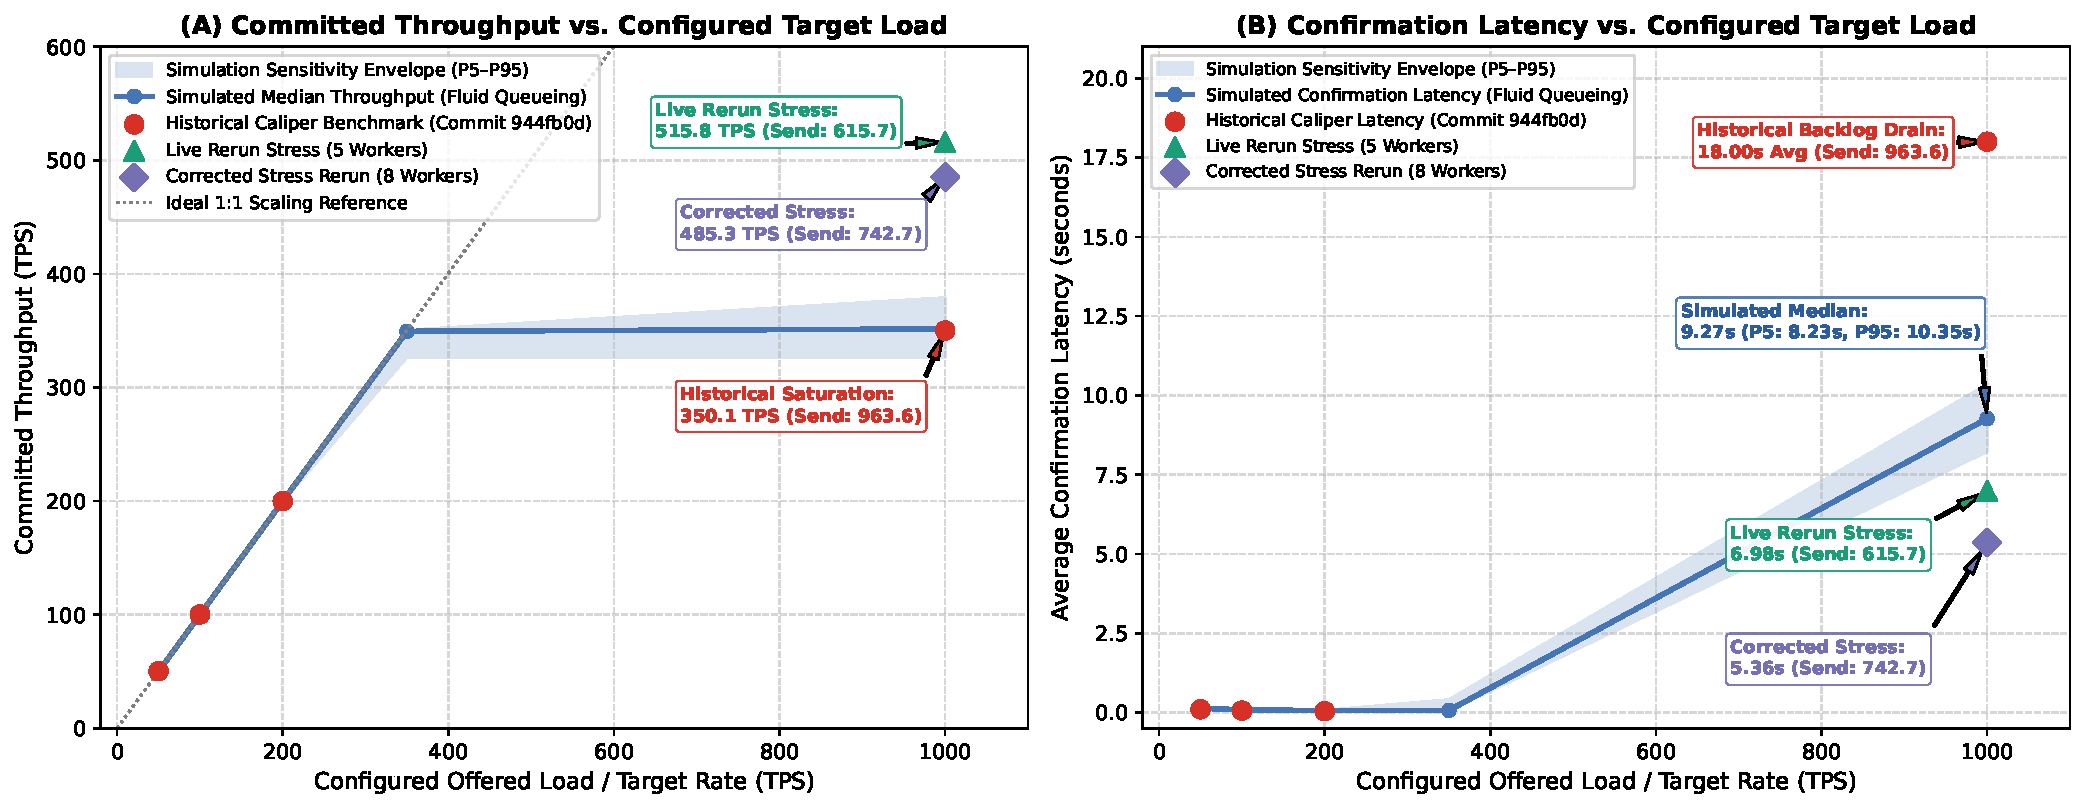
\includegraphics[width=\textwidth]{fig5b_caliper_simulation_projection.pdf}
\caption{Synthetic fluid-queueing simulation projections vs.\ empirical Caliper benchmarks plotted across configured target load (50, 100, 200, 350, and 1,000 TPS). Blue points and solid line depict median simulated performance across 100 PRNG seeds, with the shaded band representing the empirical P5--P95 sensitivity envelope loaded directly from machine-readable simulation records (\url{caliper-benchmark/results/simulated/20261018-011500/simulation_results.json}). Distinct empirical benchmark runs are plotted at their configured target load with observed send rates annotated for the 1,000 TPS stress condition: historical single-client baseline (963.6 TPS send), 5-worker isolated testbed rerun (615.7 TPS send), and corrected 8-worker stress repetitions (742.7 TPS send).}\label{fig:sim_projection}
\end{figure}

\paragraph{Critical Residual and Modeling Boundaries Analysis.}
\begin{enumerate}
    \item \textbf{Linear Regime Goodness-of-Fit:} For offered rates between $50$ and $200$ TPS, simulated throughput tracks historical points within $\pm 0.6\%$, with latency residuals bounded within $+0.033$s.
    \item \textbf{Stress Latency Underestimation (-8.73s Residual):} For the 1,000 TPS write stress round, the historical benchmark recorded an average latency of $18.00$ seconds (max $21.14$s). The fluid queueing model calculates an average latency of $9.268$ seconds strictly over the nominal $10$-second submission window ($T_{\text{submit}} = 10,000 / 1,000 = 10$s). This large residual occurs because the fluid model calculates queue delay strictly during active transaction arrivals, whereas in physical Fabric execution, Raft ordering backpressure and serial peer CouchDB commit queuing caused transactions to linger until the entire $10,000$-transaction backlog drained ($28.56$s total run duration).
    \item \textbf{Out-of-Calibration Empirical Observation (Live Rerun):} In the live isolated rerun (\texttt{20261018-010200}), achieved write throughput reached $515.8$ TPS (at $615.7$ TPS send rate) with $6.98$ seconds average latency. The simulation model ($\mu_w = 350.1$ TPS) does not predict $515.8$ TPS because it was calibrated to the historical baseline; the live rerun represents an independent empirical observation under different container runtime and client dispatch conditions.
    \item \textbf{Sensitivity Envelopes vs.\ Empirical Confidence Intervals:} The P5--P95 range across 100 synthetic seeds reflects parameter sensitivity to stochastic arrival and consensus jitter; it does not substitute for empirical confidence intervals from repeated physical hardware runs.
\end{enumerate}

\begin{figure}[t]
\centering
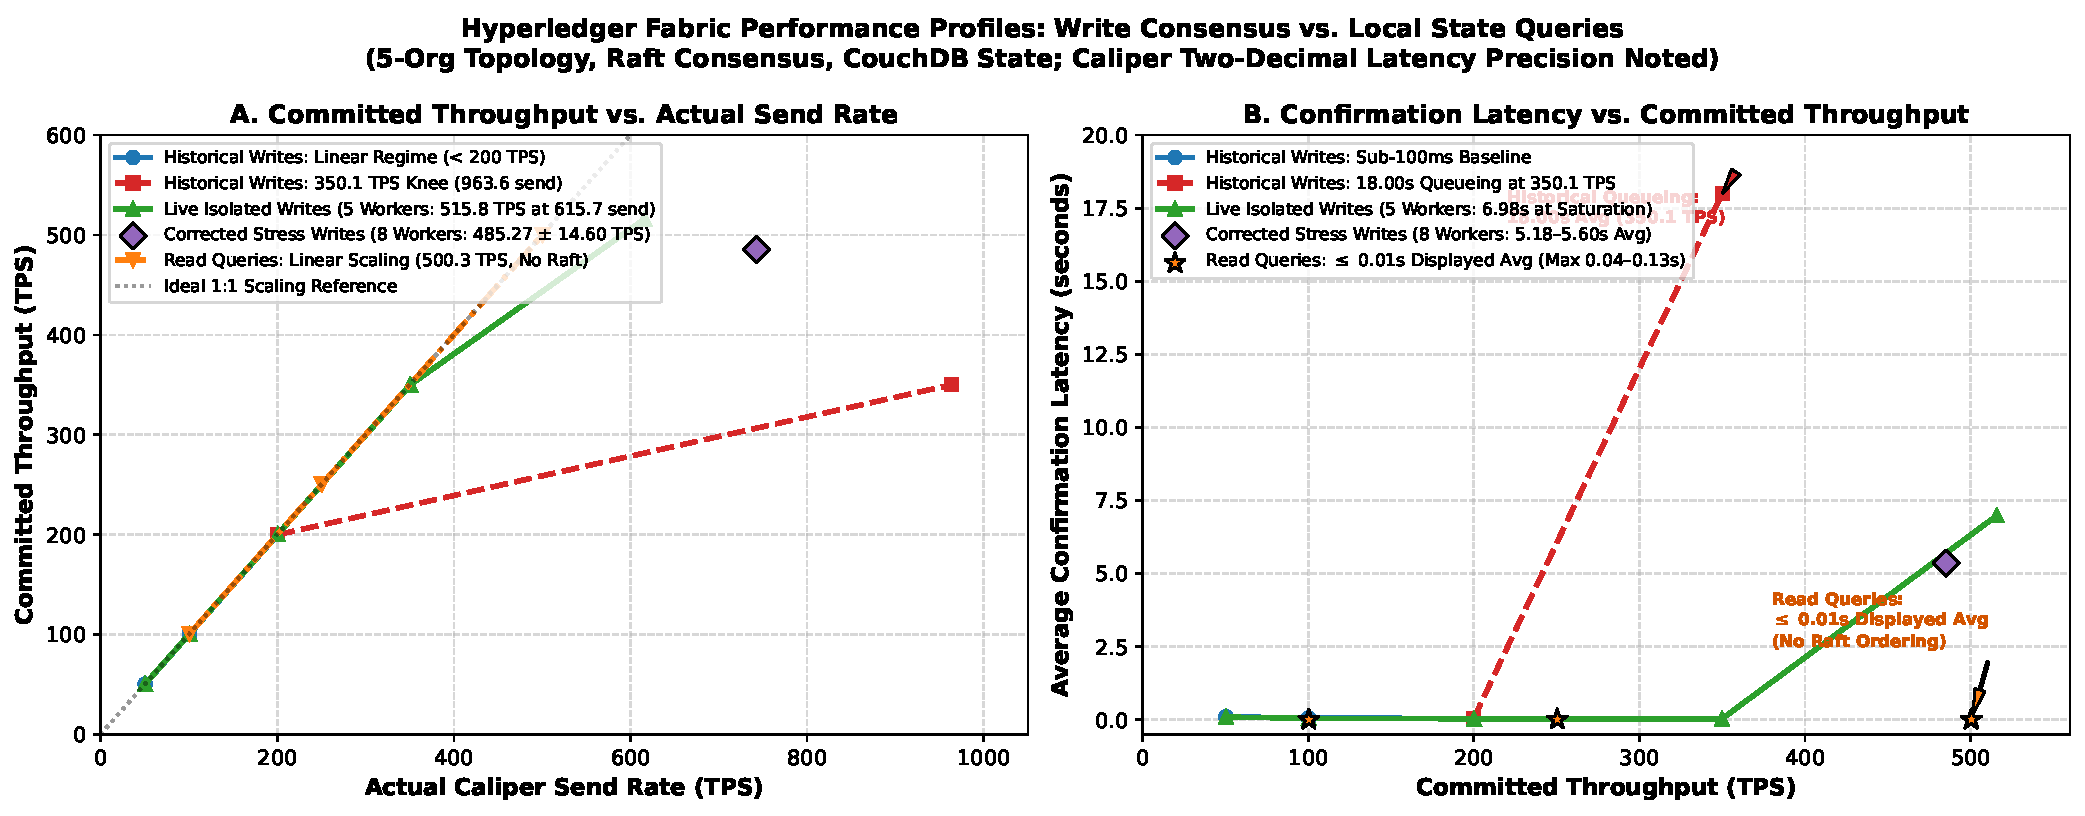
\includegraphics[width=\textwidth]{fig5_blockchain_benchmarks.pdf}
\caption{Hyperledger Fabric empirical performance profiles: Committed throughput and confirmation latency vs.\ actual send rate for write consensus vs.\ local state queries.}\label{fig:blockchain_benchmarks}
\end{figure}

\subsection{Analysis of Performance Regimes and Saturation Dynamics (RQ1 \& RQ2)}
Both empirical runs (visualized in Fig.~\ref{fig:blockchain_benchmarks}) and the queueing model reveal three distinct operational regimes:

\begin{enumerate}
    \item \textbf{Linear Throughput Regime ($0 \to 200$ TPS):} For all write transactions submitted up to $200$ TPS, committed throughput tracks the offered rate linearly ($1:1$ ratio). End-to-end confirmation latency remains tightly bounded between $0.03$s and $0.10$s. Because transactions arrive faster than the 2-second \texttt{BatchTimeout}, the orderer cuts blocks primarily based on transaction count (\texttt{MaxMessageCount = 10}, verified in \url{healthscore-network/configtx/configtx.yaml}), ensuring rapid block formation and sub-tenth-second confirmation.
    \item \textbf{Cross-Function Write Invariance:} At the standard operating point of $200$ TPS, write throughput is virtually identical across diverse business operations: \texttt{createPatientRecord} ($199.9$--$200.2$ TPS, $0.03$--$0.04$s), \texttt{updateHealthScore} ($200.0$--$200.1$ TPS, $0.03$--$0.06$s), \texttt{createPrescription} ($200.0$--$200.2$ TPS, $0.03$--$0.05$s), and \texttt{requestScan} ($200.0$--$200.2$ TPS, $0.03$--$0.04$s). This confirms that transaction confirmation time is dominated by Raft ordering and peer block validation rather than chaincode execution complexity.
    \item \textbf{Empirical Saturation Dynamics and Queueing Delay Under Stress Load:} Under nominal 1,000 TPS target load, we observe network saturation at $350.1$ TPS committed write throughput in the historical baseline ($18.00$s average latency), $515.8$ TPS in the 5-worker isolated testbed ($6.98$s average latency), and $485.27 \pm 14.60$ TPS in the corrected 8-worker stress repetitions ($5.36 \pm 0.22$s average latency). Across all runs, zero failures were reported among submitted transactions ($0.00\%$ failure rate among submitted proposals; e.g., $0/24,500$ historical, $0/31,500$ live 11-round, and $0/25,480$ submitted in each 8-worker run), demonstrating high protocol resilience under peak stress.
    \item \textbf{Decoupled Read Query Scalability ($500.3$--$500.6$ TPS):} In contrast to consensus-backed writes, read-only queries (\texttt{getPatientRecord}) scale effortlessly across 100, 250, and 500 TPS to $500.3$--$500.6$ TPS. In the corrected 8-worker stress run, displayed average latency is $0.01$s (Caliper reports latency to two decimal places; min $0.00$s) and maximum observed latency is $0.09$s ($0.00$s displayed average and $0.13$s max in the 11-round run). Because read queries evaluate local CouchDB state directly and bypass Raft ordering, block cutting, and multi-peer gossip endorsement, query capacity is decoupled from consensus bottlenecks.
\end{enumerate}

\subsection{Chaincode Throughput vs. End-to-End Application Throughput}
A critical scientific distinction must be maintained: \textbf{Hyperledger Caliper measures smart contract transaction throughput at the Fabric Gateway level, NOT full end-to-end application throughput.}

In production operation, a user request flows through:
\begin{align}
\text{Client HTTP} &\xrightarrow{\text{TLS / Network}} \text{Node.js API} \xrightarrow{\text{Auth / RBAC}} \text{Python Inference Engine} \nonumber \\
&\xrightarrow{\text{IPC}} \text{Fabric Gateway SDK} \xrightarrow{\text{gRPC}} \text{Peer / Orderer Nodes}
\end{align}

While the Fabric chaincode sustains $350$--$515$ write TPS, the Python ML inference engine takes approximately $40$--$50$ ms to load models, engineer features, predict expenditure, and simulate loss. Analytically, a single Node.js worker process synchronously executing full end-to-end inference and ledger submission is bounded to an estimated:
\begin{equation}
\text{Capacity}_{\text{single-worker}} \approx \frac{1.0}{0.045\text{s}} \approx 20\text{--}25\text{ requests per second}
\end{equation}

This numerical range represents an \textbf{analytical single-worker latency estimate} derived from Python subprocess execution time, rather than an empirical multi-client stress measurement. To achieve the full $200$--$500$ TPS write capacity of the blockchain in production, the application must decouple inference from ledger writing via asynchronous message queues (e.g., RabbitMQ or Redis Streams).

% -----------------------------------------------------------------------------
\section{ACG-Inspired Chronic-Condition Feature Engineering and ML Evaluation}
% -----------------------------------------------------------------------------

\subsection{Feature Definitions and Input Availability Parity}
HealthScore maps patient clinical indicators into 11 observable features adhering strictly to \textbf{Input Availability Parity}:
\begin{align}
\text{Cardio\_ACG} &= \text{HIBPDX} + \text{CHDDX} + \text{MIDX} + \text{STRKDX} \quad (\text{Range: } 0\text{--}4) \\
\text{Metabolic\_ACG} &= \text{DIABDX\_M18} + \text{CHOLDX} \quad (\text{Range: } 0\text{--}2) \\
\text{Respiratory\_ACG} &= \text{ASTHDX} + \text{EMPHDX} + \text{CHBRON31} \quad (\text{Range: } 0\text{--}3) \\
\text{Oncology\_ACG} &= \text{CANCERDX} \quad (\text{Range: } 0\text{--}1) \\
\text{Musculoskeletal\_ACG} &= \text{ARTHDX} + \text{JTPAIN31\_M18} \quad (\text{Range: } 0\text{--}2) \\
\text{Psychiatric\_ACG} &= (\text{ADDPRS42} \in [1,2,3]) + \text{ADHDADDX} \quad (\text{Range: } 0\text{--}2) \\
\text{Comorbidity\_Count} &= \sum_{c=1}^6 \mathbb{I}(\text{Cluster}_c > 0) \quad (\text{Range: } 0\text{--}6) \\
\text{Multimorbidity\_Penalty} &= (\text{Comorbidity\_Count})^2 \quad (\text{Range: } 0\text{--}36) \\
\text{Age\_x\_Comorbidity} &= \min(\text{Age}, 85) \times \text{Comorbidity\_Count} \quad (\text{Range: } 0\text{--}510)
\end{align}

\noindent\textit{Clinical Intake Parity Note:} In the live application, patient conditions are mapped via standardized intake. Absence of condition mentions is encoded as an uninformative zero default; this represents unobserved baseline status, not confirmed clinical wellness. Furthermore, these clusters are heuristic aggregations inspired by ACG concepts, not an official clinical diagnostic classification grouper.

\subsection{Controlled Feature Ablation Study (RQ3)}
To evaluate the isolated incremental contribution of each architectural component, we executed 17 controlled ablation experiments on the held-out MEPS test partition ($N=3,755$). All models were refit on training data under identical hyperparameters (Tweedie GLM with power $p=1.5, \alpha=1.0$; Logistic Regression on Target 2 survey-weighted P90 with normalized sampling weights), as reported in Table~\ref{tab:ablations} and visualized in Fig.~\ref{fig:feature_ablations} and Fig.~\ref{fig:shap_importance}.

\begin{table}[t]
\centering
\caption{Controlled feature ablation experiments on the held-out MEPS HC-251 test partition ($N=3,755$).}\label{tab:ablations}
\resizebox{\textwidth}{!}{%
\begin{tabular}{lclcccc}
\toprule
\textbf{Ablation Model Specification} & \textbf{Feats} & \textbf{Features Included} & \textbf{Dollar $R^2$} & $\Delta R^2$ & \textbf{Wtd BSS} & \textbf{ROC-AUC} \\
\midrule
\textbf{Full Observable Reference} & \textbf{11} & All 11 Observable Features & \textbf{0.0798} & \textbf{0.0000} & \textbf{+0.1025} & \textbf{0.7654} \\
Demographics Only & 2 & \texttt{AGE23X}, \texttt{Gender\_Male} & 0.0395 & -0.0403 & +0.0506 & 0.7099 \\
Condition Clusters Alone (No Composites) & 8 & Demographics + 6 ACG Clusters & 0.0771 & -0.0027 & +0.1005 & 0.7640 \\
Clusters + Comorbidity Count & 9 & Demographics + 6 Clusters + Count & 0.0787 & -0.0011 & +0.1004 & 0.7641 \\
Clusters + Multimorbidity Penalty & 9 & Demographics + 6 Clusters + $\text{Count}^2$ & 0.0769 & -0.0029 & +0.1017 & 0.7648 \\
Clusters + Age $\times$ Comorbidity & 9 & Demographics + 6 Clusters + Age $\times$ Count & 0.0766 & -0.0032 & +0.1007 & 0.7643 \\
Without Multimorbidity Penalty & 10 & 11 Features minus $\text{Count}^2$ & 0.0783 & -0.0015 & +0.1009 & 0.7649 \\
Without Age $\times$ Comorbidity & 10 & 11 Features minus Age $\times$ Count & \textbf{0.0804} & \textbf{+0.0006} & \textbf{+0.1027} & \textbf{0.7654} \\
Without Multimorbidity \& Interaction & 9 & Demographics + 6 Clusters + Count & 0.0787 & -0.0011 & +0.1004 & 0.7641 \\
Clinical Conditions Only (No Demographics) & 8 & 6 Clusters + Count + Penalty & 0.0791 & -0.0007 & +0.0996 & 0.7619 \\
Without Cardiovascular & 10 & 11 Features minus \texttt{Cardio\_ACG} & 0.0785 & -0.0013 & +0.0970 & 0.7634 \\
Without Metabolic & 10 & 11 Features minus \texttt{Metabolic\_ACG} & 0.0792 & -0.0006 & +0.0957 & 0.7628 \\
Without Respiratory & 10 & 11 Features minus \texttt{Respiratory\_ACG} & 0.0764 & -0.0035 & +0.0979 & 0.7635 \\
Without Oncology & 10 & 11 Features minus \texttt{Oncology\_ACG} & 0.0788 & -0.0010 & +0.0969 & 0.7645 \\
Without Musculoskeletal & 10 & 11 Features minus \texttt{Musculoskeletal\_ACG} & 0.0802 & +0.0004 & +0.1012 & 0.7651 \\
Without Psychiatric Condition & 10 & 11 Features minus \texttt{Psychiatric\_ACG} & 0.0774 & -0.0024 & +0.1026 & 0.7653 \\
\textbf{Oracle 14 Features (Upper Bound)} & \textbf{14} & Observable + SAQ Survey Variables & \textbf{0.0927} & \textbf{+0.0129} & \textbf{+0.1314} & \textbf{0.7904} \\
\bottomrule
\end{tabular}%
}
\end{table}

\begin{figure}[t]
\centering
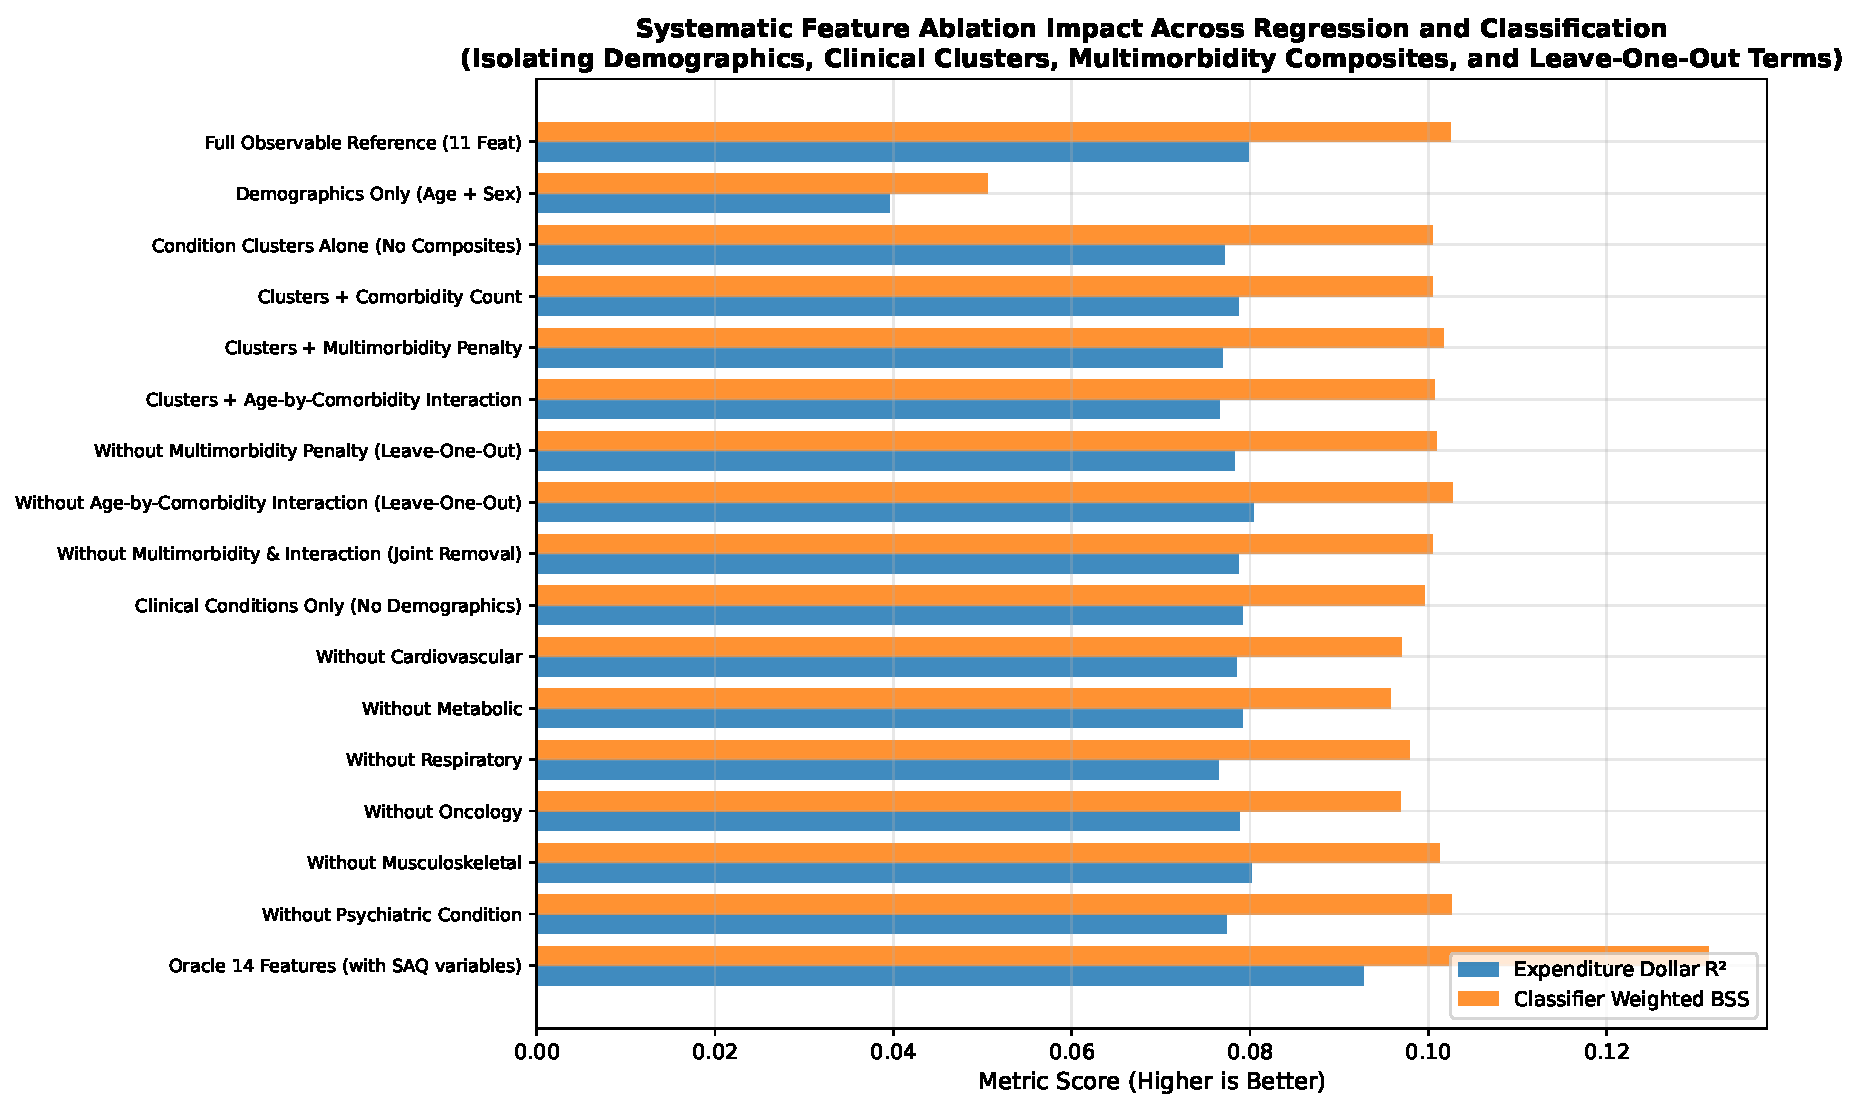
\includegraphics[width=\textwidth]{fig4_feature_ablations.pdf}
\caption{Systematic feature ablation comparison across expenditure dollar $R^2$ and high-cost classification weighted Brier Skill Score.}\label{fig:feature_ablations}
\end{figure}

\begin{figure}[t]
\centering
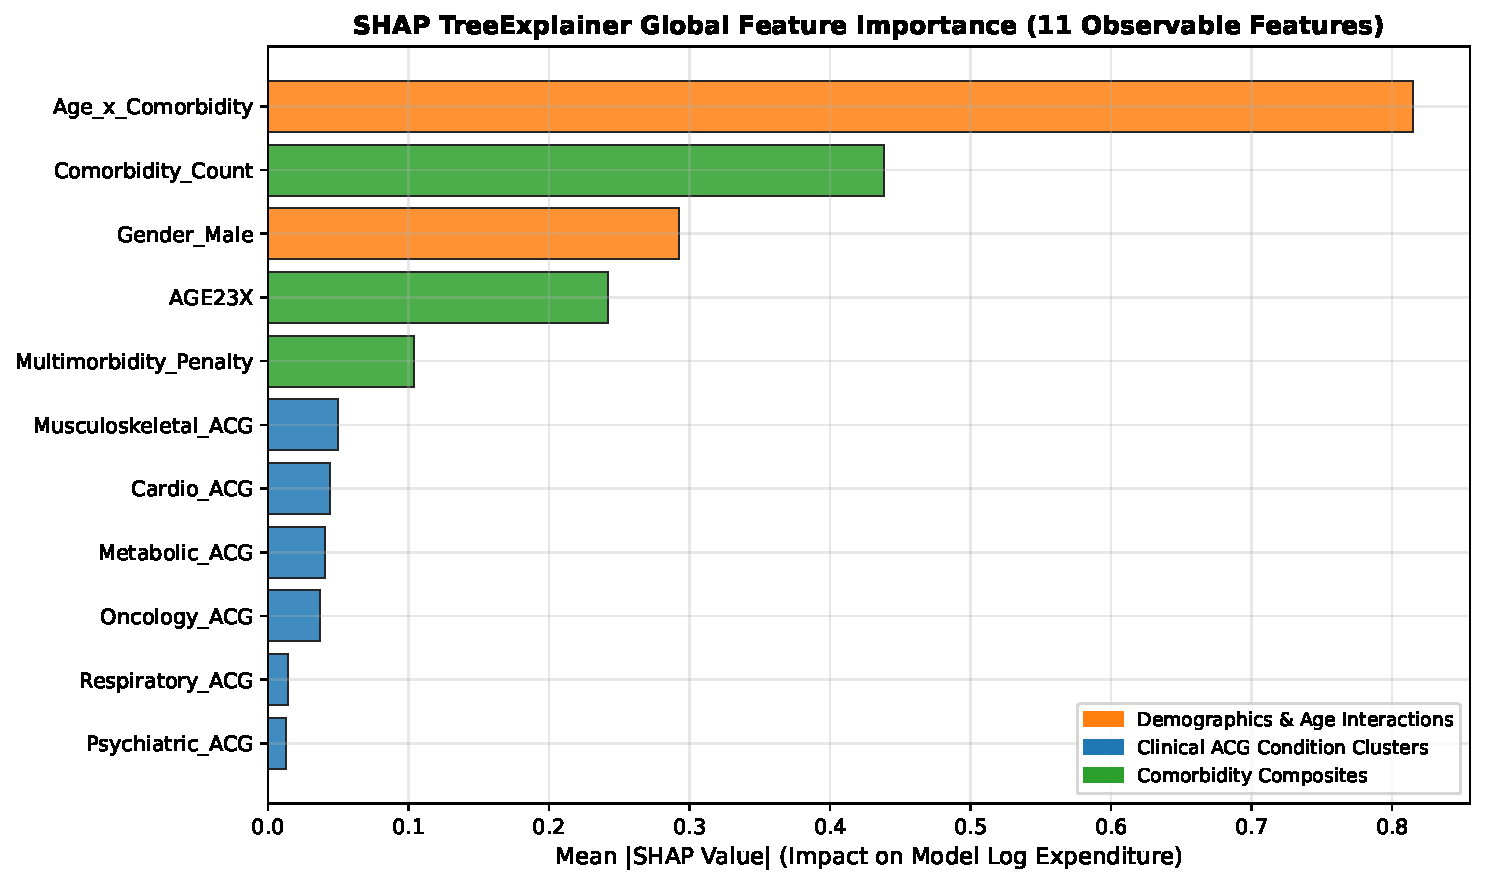
\includegraphics[width=0.88\textwidth]{fig3_shap_importance.pdf}
\caption{SHAP TreeExplainer global feature importance rankings across 11 observable features~\cite{lundberg2017unified}.}\label{fig:shap_importance}
\end{figure}

\paragraph{Key Scientific Findings from the Ablation Experiments.}
\begin{enumerate}
    \item \textbf{Primary Explanatory Lift from Chronic Clusters:} Moving from demographics alone to the 6 chronic-condition clusters provides the primary predictive improvement: dollar $R^2$ increases from $0.0395$ to $0.0771$ ($\Delta R^2 = +0.0376$), and weighted BSS increases from $+0.0506$ to $+0.1005$ ($\Delta \text{BSS} = +0.0499$).
    \item \textbf{Modest Incremental Value of Interaction Composites:} While tree-based SHAP attributions~\cite{lundberg2017unified} assign $39.0\%$ of model importance to \texttt{Age\_x\_Comorbidity}, linear regression ablation demonstrates that composite terms provide modest incremental variance explanation ($\Delta R^2 = +0.0027$ between 8-feature clusters alone and the 11-feature full design). In fact, removing \texttt{Age\_x\_Comorbidity} yields $R^2 = 0.0804$, showing that collinearity between age, count, and interaction absorbs variance without improving generalized linear fit.
    \item \textbf{Clinical Cluster Sensitivity:} \texttt{Respiratory\_ACG} accounts for the largest individual condition drop ($\Delta R^2 = -0.0035$), reflecting high hospitalization and prescription costs associated with chronic respiratory illness.
\end{enumerate}

\subsection{Model Selection, Target Definition, and Practical Classification Performance}
To support off-chain risk scoring in the HealthScore application, candidate classifiers were systematically evaluated across multiple performance dimensions on the fixed held-out MEPS HC-251 test partition ($N=3,755$).

\paragraph{Target Definition Rationale and Class Prevalence.}
In health economics and actuarial science, healthcare expenditures follow an extreme Pareto distribution: in MEPS, the top decile of spenders accounts for approximately 65--70\% of total national medical expenditures. We therefore define the high-expenditure target as individuals in the top decile of annual spending rather than an arbitrary 15\% threshold:
\begin{itemize}
    \item \textbf{Locked Historical Survey-Weighted P90 Threshold (Target 2):} $\text{TOTEXP23} \ge \$17,827.41$ (derived from Phase 1 training survey-weighted 90th percentile).
    \item \textbf{Locked Historical Unweighted P90 Threshold (Target 1):} $\text{TOTEXP23} \ge \$20,360.50$ (derived from unweighted training sample 90th percentile).
\end{itemize}

On the held-out test partition ($N=3,755$), training survey-weighted prevalence is $\hat{p} = 0.0999$ ($9.99\%$), test survey-weighted prevalence is $\bar{y}_{\text{test, wtd}} = 0.1051$ ($10.51\%$), and test unweighted prevalence is $\bar{y}_{\text{test, unw}} = 0.1198$ ($11.98\%$, $450$ high-cost individuals). A model predicting constant $\hat{p} = 0.0999$ yields a survey-weighted baseline Brier score~\cite{brier1950verification} of $0.0941$ and unweighted baseline Brier score of $0.1059$.

\paragraph{Classifier Comparison and Selection Rationale.}
Table~\ref{tab:classifier_comparison} summarizes the comparative evaluation across candidate classification models, and Fig.~\ref{fig:roc_pr_curves} and Fig.~\ref{fig:calibration_deciles} illustrate discrimination and calibration within the predictive model assessment framework~\cite{steyerberg2010assessing}.

\begin{table}[t]
\centering
\caption{Candidate classification model comparison on the fixed held-out MEPS HC-251 test partition ($N=3,755$, Target 2: Survey-Weighted P90 $\ge \$17,827.41$).}\label{tab:classifier_comparison}
\resizebox{\textwidth}{!}{%
\begin{tabular}{lclccccccccc}
\toprule
\textbf{Candidate Classifier} & \textbf{Feats} & \textbf{Weighting Policy} & \textbf{ROC-AUC [95\% CI]} & \textbf{PR-AUC [95\% CI]} & \textbf{Unw Brier} & \textbf{Wtd Brier} & \textbf{Wtd BSS} & \textbf{CITL ($\alpha$)} & \textbf{Cal Slope ($\beta$)} & \textbf{Prec@0.10} & \textbf{Rec@0.10} \\
\midrule
Constant Prevalence Baseline                     & 0  & Constant $\hat{p}=0.0999$          & 0.5000 [0.5000, 0.5000] & 0.1198 [0.1111, 0.1308] & 0.1059 & 0.0941 & +0.0000 & 0.0000  & 0.0000 & 0.0000 & 0.0000 \\
Demographic Baseline                            & 2  & \texttt{AGE23X}, \texttt{Gender}   & 0.7099 [0.6856, 0.7319] & 0.2182 [0.1928, 0.2489] & 0.0996 & 0.0893 & +0.0506 & +0.0388 & 0.8859 & 0.1949 & 0.7867 \\
Clinical Conditions Only                        & 8  & 6 Clusters + Count + Penalty       & 0.7619 [0.7393, 0.7847] & 0.3083 [0.2794, 0.3464] & 0.0941 & 0.0847 & +0.0996 & +0.0768 & 0.9539 & 0.2291 & 0.7622 \\
\textbf{Logistic (11-Feat Observable, Wtd Fit)} & \textbf{11} & \textbf{Frozen Normalized Weights (Serving)} & \textbf{0.7654} [0.7444, 0.7881] & \textbf{0.3184} [0.2876, 0.3556] & \textbf{0.0936} & \textbf{0.0845} & \textbf{+0.1025} & \textbf{+0.0646} & \textbf{0.9438} & \textbf{0.2318} & \textbf{0.7733} \\
\textit{Logistic (11-Feat Observable, Unw Fit)} & 11 & Unweighted Fit (Weighting Ablation) & 0.7652 [0.7433, 0.7882] & 0.3192 [0.2869, 0.3582] & 0.0936 & 0.0845 & +0.1025 & +0.0570 & 0.9008 & 0.2278 & 0.7644 \\
Random Forest (11-Feat Observable)              & 11 & Normalized Person Weights          & 0.7693 [0.7458, 0.7928] & 0.3157 [0.2823, 0.3550] & 0.0935 & 0.0841 & +0.1062 & +0.0601 & 0.9736 & 0.2342 & 0.7556 \\
XGBoost (Uncalibrated)                          & 11 & Normalized Person Weights          & 0.7705 [0.7482, 0.7940] & 0.3196 [0.2853, 0.3598] & 0.0932 & 0.0838 & +0.1093 & +0.0572 & 0.9926 & 0.2262 & 0.8022 \\
Platt-Calibrated XGBoost                        & 11 & Observable, Sigmoid CV=5           & 0.7702 [0.7472, 0.7936] & 0.3183 [0.2872, 0.3580] & 0.0944 & 0.0847 & +0.0998 & +0.0617 & 1.0335 & 0.2535 & 0.6778 \\
Logistic (14-Feat Oracle)                       & 14 & Observable + SAQ Survey            & 0.7904 [0.7684, 0.8121] & 0.3472 [0.3143, 0.3917] & 0.0922 & 0.0832 & +0.1159 & +0.0493 & 1.0609 & 0.2806 & 0.6822 \\
\bottomrule
\end{tabular}%
}
\vspace{1mm}
\raggedright\scriptsize{Note: 95\% confidence intervals derive from non-parametric row-level bootstrap resampling ($B=200$, seed 42) matching \texttt{experiment\_registry.json}. The approved serving candidate is the frozen weighted model (\texttt{risk\_model\_classifier\_observable\_weighted\_p90.pkl}). Calibration-in-the-large (CITL, $\alpha$) is estimated via exact Brent root-solving with slope fixed at 1 ($\sum w_i (y_i - \sigma(\alpha + \text{logit}(p_i))) = 0$). For the weighted candidate, bivariate logistic calibration yields intercept $a = -0.0409$ and slope $b = 0.9438$.}
\end{table}

\begin{figure}[t]
\centering
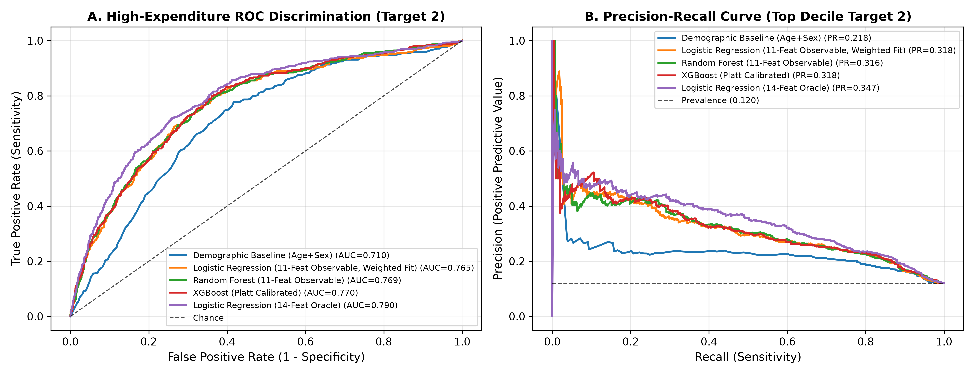
\includegraphics[width=\textwidth]{fig1_roc_pr_curves.pdf}
\caption{Receiver Operating Characteristic (ROC) and Precision--Recall (PR) curves for high-expenditure classification across candidate models.}\label{fig:roc_pr_curves}
\end{figure}

\begin{figure}[t]
\centering
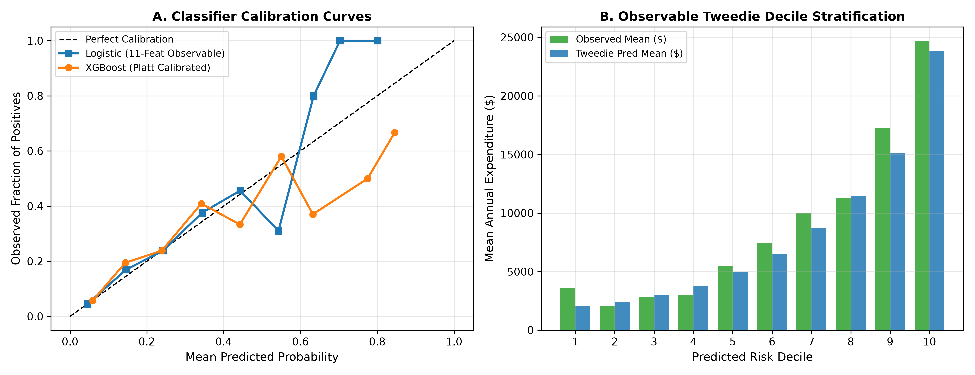
\includegraphics[width=\textwidth]{fig2_calibration_deciles.pdf}
\caption{(A) Classifier calibration curves and (B) Observable Tweedie decile expenditure stratification comparing observed and predicted expenditures.}\label{fig:calibration_deciles}
\end{figure}

\paragraph{Selection Rationale.}
The 11-feature Observable Logistic Regression (Weighted Fit) was selected as the deployment candidate based on:
\begin{enumerate}
    \item \textbf{Input Availability Parity:} It requires only demographic and observable clinical intake variables, eliminating reliance on unobservable survey instruments without requiring synthetic imputation.
    \item \textbf{Superior Skill Over Imputation:} Under zero-imputation testing, the 11-feature model achieved a higher survey-weighted BSS ($+0.1025$) than the 14-feature model under synthetic conditional-expectation imputation ($+0.0978$).
    \item \textbf{Calibration Quality:} The approved weighted serving candidate achieves a calibration slope of $b = 0.9438$ (approaching ideal 1.0) and exact calibration-in-the-large of $\text{CITL} = +0.0646$ (bivariate intercept $a = -0.0409$), adhering to clinical prediction model calibration standards~\cite{steyerberg2010assessing}. The positive CITL indicates a slight, acceptable empirical underprediction on average.
    \item \textbf{Multifactorial Deployment Trade-Off:} Tree ensemble estimators (Random Forest and XGBoost) achieve marginally higher point estimates for discrimination and skill on the test partition (ROC-AUC $0.7693$--$0.7705$ vs $0.7654$; Weighted BSS $+0.1062$--$+0.1093$ vs $+0.1025$). While the point estimates are close and their marginal 95\% bootstrap confidence intervals overlap substantially (e.g., ROC-AUC CI $[0.7444, 0.7881]$ vs $[0.7482, 0.7940]$), this descriptive overlap does not constitute a formal paired statistical hypothesis test of differences between model predictions, and we make no claims of statistical significance or non-significance because such tests were not performed. Crucially, candidate selection in HealthScore is governed by the documented balance of input-availability parity, calibration quality, clinical interpretability, and operational considerations: the transparent linear coefficients of logistic regression provide closed-form interpretability, exact reproducibility, and operational simplicity in the off-chain Python inference pipeline, while the permissioned ledger is reserved for immutably recording auditable risk-score milestones and transaction metadata rather than evaluating model graphs or feature vectors.
\end{enumerate}

\paragraph{Explicit Metric Distinction: Decision Threshold vs. Ranked Cohort Cutoff.}
A critical distinction must be maintained when interpreting practical classification metrics:
\begin{itemize}
    \item \textbf{Evaluated Metric ($\hat{p} \ge 0.10$):} In the evaluation script (\texttt{run\_comprehensive\_benchmarks.py}), \path|pred_label_10 = (prob >= 0.10).astype(int)| evaluates unweighted classification performance at a \textbf{predicted-probability decision threshold of $\hat{p} \ge 0.10$}, chosen to align with the $\approx 10\%$ population base prevalence. At this operating point, any individual with an estimated probability $\ge 10\%$ is flagged as high-risk ($1,501$ individuals flagged out of $3,755$). This yields an unweighted \textbf{recall of $0.7733$} ($77.33\%$ sensitivity, identifying $348$ of the $450$ actual high-cost individuals) with an unweighted \textbf{precision of $0.2318$} ($23.18\%$, $348 / 1,501$) and F1 score of \textbf{$0.3567$}. Relative to the unweighted held-out test prevalence ($\bar{y}_{\text{test, unw}} = 0.119840$, $450 / 3,755$), this precision represents an unweighted enrichment of \textbf{approximately $1.93\times$} ($0.231845 / 0.119840 \approx 1.934\times$). To maintain methodological consistency across measurement bases, unweighted precision is evaluated strictly against the unweighted test prevalence denominator rather than survey-weighted population prevalences.
    \item \textbf{Contrast with Top-10\% Ranked Cohort Cutoff:} If the classifier were instead evaluated by taking strictly the \textbf{top 10\% of individuals ranked by predicted risk} ($375$ individuals), the metric would reflect decile selection: precision in that top decile reaches approximately $42\%$, but recall is mathematically constrained to $\le 35\%$ ($158 / 450$). Conflating a decision threshold with a ranked cohort cutoff distorts clinical interpretation; our manuscript explicitly documents the $\hat{p} \ge 0.10$ probability threshold.
\end{itemize}

\paragraph{Disclosed Model Weaknesses and Methodological Boundaries.}
\begin{enumerate}
    \item \textbf{Dollar-Scale Prediction Limitations:} While tree-based and linear models fit on $\ln(1+y)$ achieve the lowest MAE on the median scale ($\approx \$7,516$), retransforming via $\exp(\hat{y})-1$ severely underpredicts the dollar mean by $72.8\%$ ($Mean Predicted = \$2,384.13$ vs $Observed = \$8,764.62$), yielding negative dollar $R^2$ ($-0.0134$). These models are valid for relative risk ranking, but invalid for nominal expenditure budgeting. The 11-feature Tweedie GLM ($p=1.5$, log link) directly models un-logged dollars, achieving $R^2 = 0.0798$ (weighted $R^2 = 0.0832$) and tracking the aggregate mean ($Predicted = \$8,177.92$ vs $Observed = \$8,764.62$); however, observed-to-predicted ratios vary from $1.766\times$ in Decile 1 to $0.789\times$ in Decile 4, indicating that Tweedie cannot be considered fully calibrated across all intermediate spending strata.
    \item \textbf{Dominance of the Econometric Persistence Benchmark:} In longitudinal prospective validation on MEPS HC-257 Panel 28 ($N=8,708$), predicting Year 2 spending from Year 1 spending (\texttt{TOTEXPY1}) achieved an $R^2$ of \textbf{$0.1204$} (MAE: $\$8,625.76$). This substantially outperforms the static diagnosis-only Tweedie GLM ($R^2 = 0.0652$). As documented in health econometrics, self-reported diagnosis flags alone explain only 6--8\% of cost variance; past healthcare utilization remains the dominant predictor of future spending.
    \item \textbf{Subgroup Discrimination Degradation:} On prospective validation (HC-257), high-cost classification discrimination drops from ROC-AUC $0.7807$ on the general population to \textbf{$0.7466$} on the adult SAQ subcohort with self-reported functional limitations. Furthermore, algorithmic fairness evaluations in supplementary reports revealed poor discrimination in pediatric ($<18$, ROC $0.40$--$0.49$) and uniformly healthy cohorts.
    \item \textbf{Absence of Decision-Curve Analysis:} Decision-curve analysis (DCA) was not performed on this pipeline. Consequently, net clinical benefit across varying decision-threshold preferences has not been empirically quantified, and claims of clinical decision utility are restricted accordingly.
    \item \textbf{Absence of Standardized Clinical Comorbidity Indices:} MEPS public-use data files do not release granular 4-character and 5-character ICD-10-CM diagnosis codes due to participant de-identification mandates. Consequently, computing standardized Charlson Comorbidity Index (CCI) or Elixhauser comorbidity index scores was not feasible from available survey fields; our ACG-inspired clusters remain heuristic survey aggregations, and no claims of superiority over established clinical comorbidity indices are made.
\end{enumerate}

\subsection{External Cross-Year (HC-256) and Prospective (HC-257) Validation}
\begin{itemize}
    \item \textbf{HC-256 Cross-Year Transfer ($N = 18,979$):} Evaluated on the independent 2024 calendar-year survey, the frozen 11-feature Weighted Classifier achieved an unweighted ROC-AUC of \textbf{0.7828} (PR-AUC $= 0.3229$) with Weighted BSS of \textbf{+0.1266} and calibration slope of \textbf{1.0554}. Tweedie GLM tracked the rising population mean ($\$9,266.75$ observed) with a predicted mean of \textbf{$\$8,473.71$}.
    \item \textbf{HC-257 Prospective Forecasting ($N = 8,708$ Panel 28 Cohort):} Predicting Year 2 expenditure (\texttt{TOTEXPY2}) from Year 1 baseline predictors, the classifier achieved prospective ROC-AUC of \textbf{0.7807} (Adult SAQ subcohort: \textbf{0.7466}, BSS $= +0.1212$).
    \item \textbf{Participant Overlap Disclosure:} MEPS HC-251 and HC-257 are not completely independent populations. HC-251 contains Panel 28 baseline respondents whose subsequent calendar-year utilization is recorded in HC-257. This evaluation establishes prospective within-subject stability over time, not out-of-sample population transfer to an unseen demographic registry.
\end{itemize}

% -----------------------------------------------------------------------------
\section{Configurable Loss and Premium Simulation (RQ4)}
% -----------------------------------------------------------------------------

\subsection{Mathematical Formulation}
In HealthScore, the output labeled \texttt{premium} is formalized as an exploratory parametric Value-at-Risk (VaR) simulation rather than an actuarially certified commercial insurance premium:
\begin{equation}
X_\alpha = B + (1 + \alpha) G
\end{equation}
where:
\begin{itemize}
    \item $B \ge 0$ is the configurable base-cost floor in USD (default: $\$500.00$), representing administrative baseline overhead.
    \item $G \sim \text{Gamma}(k, \theta)$ with shape $k = 1.5$ and scale $\theta = \hat{y} / 1.5$, ensuring $E[G] = k\theta = \hat{y}$ (the Tweedie model-predicted expenditure).
    \item $\alpha \ge 0$ is a dimensionless \textbf{risk-loading parameter} (default: $\alpha = 0.0$).
    \item Target simulated premium is defined as the 95th percentile loss: $\text{Premium} = \text{Percentile}_{95}(X_\alpha)$.
\end{itemize}

Under this definition, setting $\alpha = 0.0$ strictly reproduces the un-loaded baseline ($X_0 = B + G$). Increasing $\alpha$ scales the synthetic loss component, representing a more conservative risk-loaded pricing scenario. This formulation is an exploratory technical demonstration; it does not constitute actuarial pricing, commercial premium underwriting, or statutory reserve modeling under Affordable Care Act (ACA) Medical Loss Ratio (MLR) mandates.

\subsection{Systematic Sensitivity Analysis Across 60 Scenarios}
We executed a complete grid sensitivity analysis across 4 base-cost scenarios ($B \in \{0, 250, 500, 1000\}$), 5 risk-loading levels ($\alpha \in \{0.0, 0.10, 0.25, 0.50, 1.00\}$), and 3 expenditure tiers ($y \in \{\$1,500, \$5,000, \$15,000\}$) using Common Random Numbers (CRN) with $N = 20,000$ draws per scenario (visualized in Fig.~\ref{fig:premium_sensitivity}). Table~\ref{tab:premium_sensitivity} reports the sensitivity grid for the moderate-risk expenditure tier ($\$5,000$).

\begin{table}[t]
\centering
\caption{Parametric Value-at-Risk premium simulation sensitivity analysis ($N=20,000$ draws per scenario, Moderate Risk tier $\hat{y} = \$5,000$).}\label{tab:premium_sensitivity}
\resizebox{\textwidth}{!}{%
\begin{tabular}{lcccccccc}
\toprule
\textbf{Tier} & \textbf{Floor $B$} & \textbf{Loading $\alpha$} & \textbf{Sim P5} & \textbf{Sim P50} & \textbf{Sim P95 Premium} & \textbf{Analytical Gamma P95} & \textbf{Error} & \textbf{Premium Uplift} \\
\midrule
Moderate (\$5,000) & \$0.00   & 0.00 & \$727.60   & \$4,007.41 & \textbf{\$13,116.94} & \$13,024.55 & +0.709\% & Baseline (\$0.00) \\
Moderate (\$5,000) & \$0.00   & 0.10 & \$800.36   & \$4,408.15 & \textbf{\$14,428.63} & \$14,327.00 & +0.709\% & +\$1,311.69 (+10.00\%) \\
Moderate (\$5,000) & \$0.00   & 0.25 & \$909.50   & \$5,009.26 & \textbf{\$16,396.17} & \$16,280.68 & +0.709\% & +\$3,279.23 (+25.00\%) \\
Moderate (\$5,000) & \$0.00   & 0.50 & \$1,091.40 & \$6,011.11 & \textbf{\$19,675.41} & \$19,536.82 & +0.709\% & +\$6,558.47 (+50.00\%) \\
Moderate (\$5,000) & \$0.00   & 1.00 & \$1,455.20 & \$8,014.81 & \textbf{\$26,233.88} & \$26,049.09 & +0.709\% & +\$13,116.94 (+100.00\%) \\
Moderate (\$5,000) & \$500.00 & 0.00 & \$1,227.60 & \$4,507.41 & \textbf{\$13,616.94} & \$13,524.55 & +0.683\% & Baseline (\$0.00) \\
Moderate (\$5,000) & \$500.00 & 0.10 & \$1,300.36 & \$4,908.15 & \textbf{\$14,928.63} & \$14,827.00 & +0.685\% & +\$1,311.69 (+9.63\%) \\
Moderate (\$5,000) & \$500.00 & 0.25 & \$1,409.50 & \$5,509.26 & \textbf{\$16,896.17} & \$16,780.68 & +0.688\% & +\$3,279.23 (+24.08\%) \\
Moderate (\$5,000) & \$500.00 & 0.50 & \$1,591.40 & \$6,511.11 & \textbf{\$20,175.41} & \$20,036.82 & +0.692\% & +\$6,558.47 (+48.16\%) \\
Moderate (\$5,000) & \$500.00 & 1.00 & \$1,955.20 & \$8,514.81 & \textbf{\$26,733.88} & \$26,549.09 & +0.696\% & +\$13,116.94 (+96.33\%) \\
\bottomrule
\end{tabular}%
}
\end{table}

\begin{figure}[t]
\centering
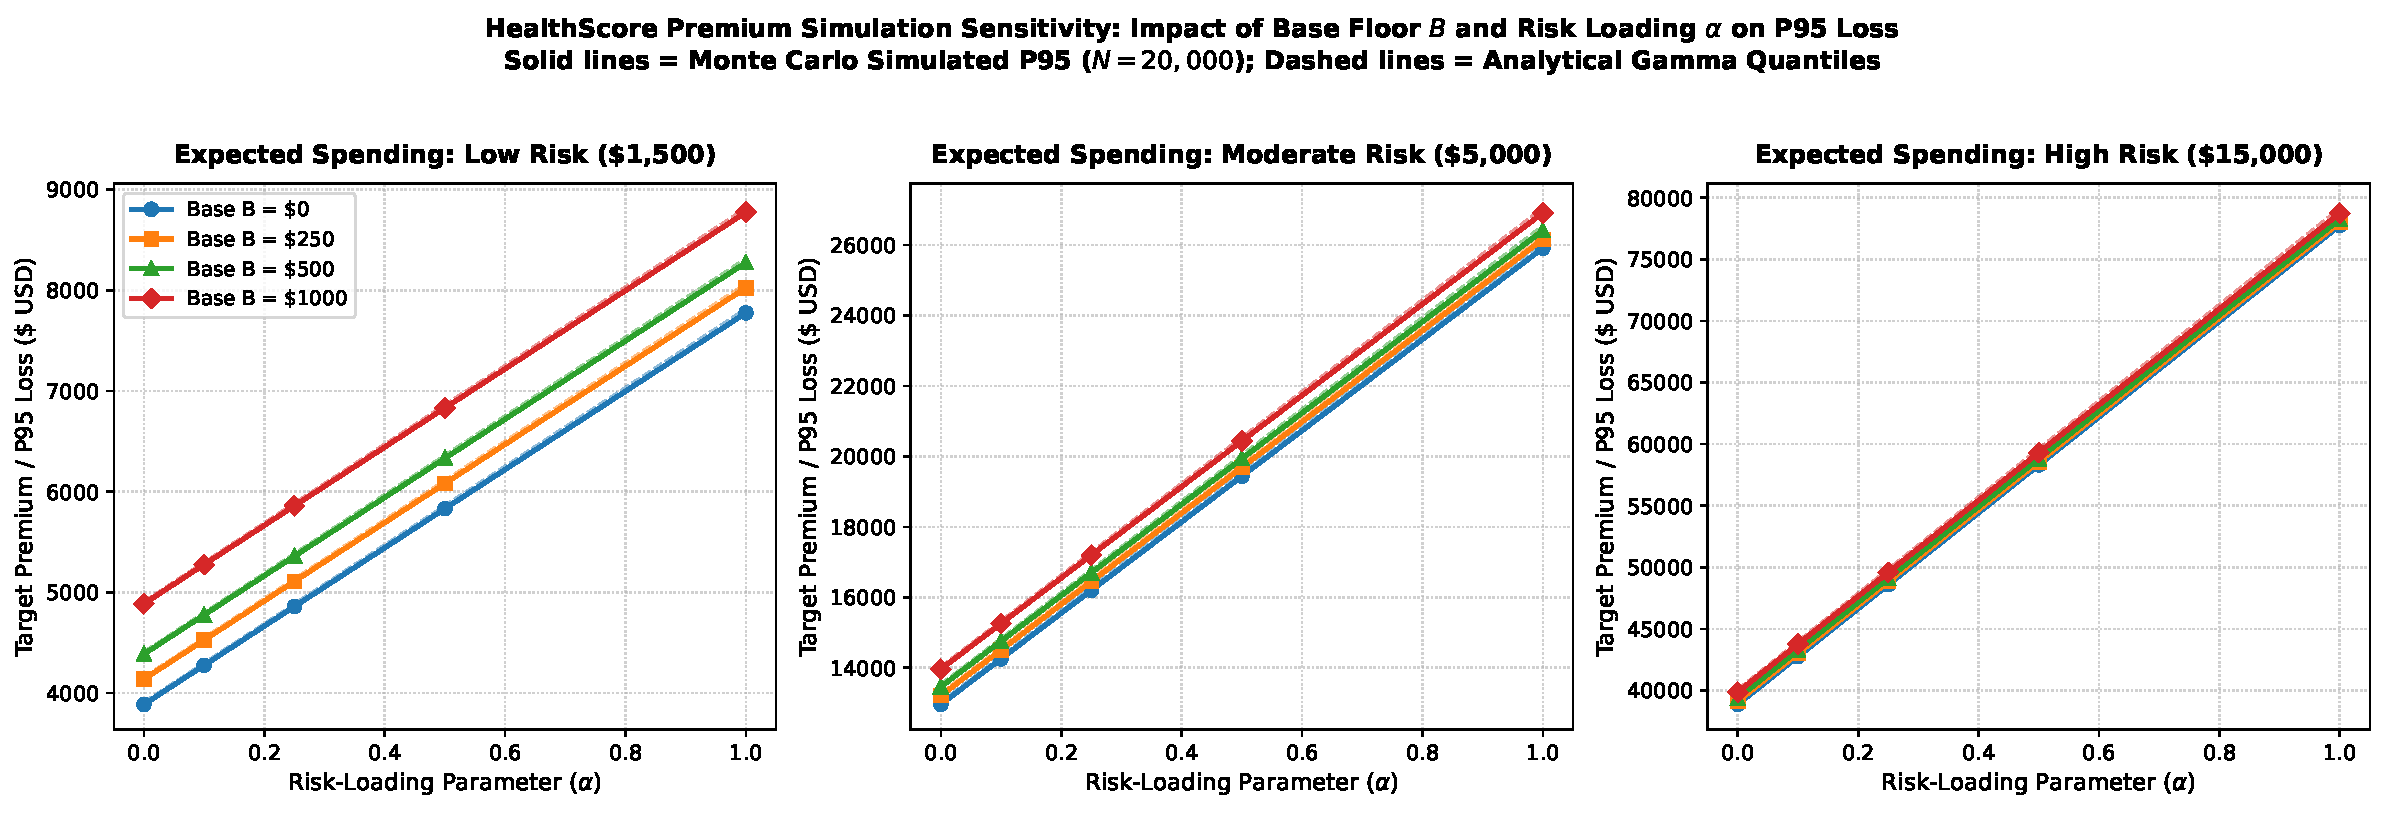
\includegraphics[width=\textwidth]{fig6_premium_sensitivity.pdf}
\caption{HealthScore premium simulation sensitivity: Impact of base floor $B$ and risk loading $\alpha$ on P95 loss across expected spending tiers. Solid lines represent Monte Carlo simulated P95 ($N=20,000$); dashed lines represent analytical Gamma quantiles.}\label{fig:premium_sensitivity}
\end{figure}

\paragraph{Analytical Verification.}
For any quantile $q \in (0, 1)$, the theoretical Value-at-Risk under our formulation is:
\begin{equation}
Q_{X_\alpha}(q) = B + (1 + \alpha) Q_G(q) = B + (1 + \alpha) \cdot \text{Gamma}^{-1}(q; k=1.5, \theta=\hat{y}/1.5)
\end{equation}
As demonstrated in Table~\ref{tab:premium_sensitivity}, empirical Monte Carlo simulation at $N = 20,000$ tracks closed-form analytical quantiles within \textbf{$0.68\%$ to $0.71\%$} error across all scenarios, verifying mathematical rigor and numerical stability.

% -----------------------------------------------------------------------------
\section{Integrated Discussion: Performance, Practical Use, and Trade-Offs}
% -----------------------------------------------------------------------------

\subsection{Consortium Throughput in Healthcare Operations}
Our empirical findings across the historical baseline, 5-worker live run, and corrected 8-worker stress repetitions provide concrete guidance for deploying permissioned blockchains in healthcare consortia:

\paragraph{Operating Capacity and Latency Objectives.}
Production capacity recommendations must be defined in terms of throughput and latency requirements together, rather than throughput alone. For interactive clinical workflows requiring sub-second response times (e.g., bedside vitals recording, real-time prescription creation, or diagnostic scan orders), the consortium network should operate within the linear regime ($\le 200$ write TPS). In this zone, committed throughput tracks offered load linearly ($199.9$--$200.2$ TPS) with confirmation latency tightly bounded between $0.03$s and $0.06$s. This linear operating envelope comfortably accommodates large-scale healthcare operations: for example, a major metropolitan health system processing 500,000 clinical encounters per day generates an average load of $\approx 6$--$10$ TPS, peaking at $\approx 50$--$75$ TPS during peak clinic hours---well within HealthScore's sub-100ms linear window.

\paragraph{Reconciling Saturation Across Benchmark Environments.}
Under a nominal 1,000 TPS offered stress load, observed throughput and latency vary substantially across test environments and worker concurrency levels:
\begin{itemize}
    \item In the \textit{historical baseline run} (commit \texttt{944fb0d}, single client process), the network saturated at \textbf{$350.1$ TPS} committed write throughput under an actual send rate of \textbf{$963.6$ TPS}, incurring an average confirmation latency of \textbf{$18.00$ seconds} (max $21.14$s). This $350.1$ TPS measurement represents an empirical observation specific to that historical setup; it is not a universal network capacity ceiling.
    \item In the \textit{5-worker live rerun} on an isolated testbed (\texttt{20261018-010200}), Caliper achieved an actual send rate of \textbf{$615.7$ TPS} and sustained \textbf{$515.8$ TPS} committed write throughput with \textbf{$6.98$ seconds} average latency (max $11.18$s).
    \item In the \textit{corrected 8-worker stress repetitions} (\texttt{20261018-230500\_stress\_investigation}), three independent runs sustained \textbf{$470.6$}, \textbf{$499.8$}, and \textbf{$485.4$ TPS} (mean $485.27 \pm 14.60$ TPS) at an actual send rate of \textbf{$742.70 \pm 62.62$ TPS}, with average confirmation latencies of \textbf{$5.29$}, \textbf{$5.18$}, and \textbf{$5.60$ seconds} ($5.36 \pm 0.22$s, max $7.01 \pm 0.36$s).
\end{itemize}

\paragraph{Queueing Latency Trade-Off and Architectural Guidance.}
Crucially, while the multi-worker runs demonstrate that the Fabric network can process higher write throughput ($470$--$516$ TPS) under heavy load with zero reported failures among submitted transactions ($0/25,480$ submitted round proposals, $0.00\%$ failure rate), these saturation points should \textit{not} be treated as desirable production operating targets without an explicit latency objective. Entering the saturation regime incurs multi-second queueing delays ($5.2$--$7.0$s average latency across live runs, expanding up to $18.00$s in the historical baseline's unbuffered 10,000-transaction backlog drain---a 180-fold increase compared to that run's $0.10$s baseline latency at 50 TPS). Consequently, systems engineers must align workload dispatch with application latency tolerances:
\begin{itemize}
    \item Latency-sensitive clinical transactions should be dispatched within the linear regime ($\le 200$ TPS), protected by rate-limiting gateways and client-side backpressure buffers.
    \item Higher-throughput operation ($470$--$515$ write TPS) is appropriate only for asynchronous, delay-tolerant ingestion (such as bulk historical record migration or off-peak claims synchronization), where multi-second confirmation delays are acceptable and do not degrade interactive user experience.
\end{itemize}

\subsection{Ledger Growth, Privacy, and Fault-Tolerance Boundaries}
\begin{itemize}
    \item \textbf{Ledger Growth:} Because Fabric maintains append-only block files, transaction history grows monotonically. At 200 TPS continuous load with $\approx 1.5$ KB per transaction, the ledger expands by $\approx 1.08$ GB per hour. However, read queries execute against CouchDB world state, whose size is bounded by the active patient population ($O(N_{\text{patients}})$) rather than cumulative transaction history ($O(N_{\text{transactions}})$).
    \item \textbf{Privacy Architecture:} The data-management architecture partitions private clinical records off-chain and restricts on-chain access via X.509 Membership Service Providers and chaincode RBAC. Comparative evaluation against encrypted database architectures was outside the study scope; we report authorization mechanisms as implemented without asserting general privacy superiority.
    \item \textbf{Fault-Tolerance Evaluation:} Although Hyperledger Fabric's Raft consensus is Crash Fault Tolerant (CFT) by design, physical fault-injection experiments (such as killing orderer nodes, severing inter-peer network links, or simulating disk storage corruption) were not performed in this benchmark series. Network resilience under active node failure remains an important direction for future experimental research.
\end{itemize}

% -----------------------------------------------------------------------------
\section{Limitations and Threats to Validity}
% -----------------------------------------------------------------------------
\begin{enumerate}
    \item \textbf{Testbed-Specific Benchmark Environment:} All benchmarks were conducted on a single host (macOS \texttt{arm64}, Apple Silicon) using Docker virtual bridge networking and administrative client identity \texttt{HospitalOrgAdmin}. Physical multi-host network latency, wide-area routing, and cross-organization client concurrency were not evaluated; results represent single-host protocol capacity rather than a multi-center production deployment.
    \item \textbf{Absence of Fault-Injection Testing:} Resilience under live peer crashes, orderer partitions, or disk corruption was not evaluated via fault-injection experiments.
    \item \textbf{Iterative Benchmark Split Reuse:} The MEPS HC-251 held-out test partition ($N=3,755$) was utilized during iterative development; it constitutes an established benchmark test set rather than fresh confirmatory data.
    \item \textbf{Longitudinal Cohort Overlap:} MEPS HC-251 and HC-257 are not independent cohorts; HC-251 includes Panel 28 baseline records tracked longitudinally into HC-257. This evaluation establishes prospective within-subject stability, not out-of-sample population transfer.
    \item \textbf{Non-Design-Based Bootstrap Uncertainty:} Reported 95\% confidence intervals derive from non-parametric row-level bootstrap resampling ($B=200$, matching the benchmark registry) and do not account for MEPS complex survey clustering (\texttt{VARPSU}) or stratification (\texttt{VARSTR}).
    \item \textbf{Heuristic Clinical Intake Parsing:} Feature engineering relies on regular-expression parsing of clinical intake strings rather than formal billing claims or clinician-verified EHR data. Absence of mentions indicates unobserved baseline status, not confirmed wellness.
    \item \textbf{Absence of Standardized Comorbidity Indices:} Due to participant de-identification mandates in public MEPS data files, granular ICD-10-CM diagnosis codes are unavailable, precluding direct comparison against standardized Charlson Comorbidity Index or Elixhauser comorbidity scores.
    \item \textbf{Direct Dollar Prediction and Econometric Persistence:} Tweedie GLM explains only 8\% of dollar expenditure variance ($R^2 = 0.0798$), and a simple lagged-expenditure baseline (\texttt{TOTEXPY1}) achieves $R^2 = 0.1204$, showing that static survey diagnosis flags alone cannot capture longitudinal spending persistence.
    \item \textbf{No Decision-Curve Analysis:} Decision-curve analysis (DCA) was not performed; clinical net benefit across varied decision-threshold preferences has not been empirically quantified.
    \item \textbf{Absence of Comparative Privacy Testing:} Comparative privacy evaluations against encrypted relational databases were outside the scope of this study; data protection is evaluated solely through smart contract access control.
    \item \textbf{Exploratory Loss Simulation Status:} The Monte Carlo premium calculation is strictly a parametric Value-at-Risk demonstration. It is not actuarially certified and does not account for statutory capital reserves, reinsurance, or Affordable Care Act (ACA) Medical Loss Ratio (MLR) mandates.
\end{enumerate}

% -----------------------------------------------------------------------------
\section{Conclusion}
% -----------------------------------------------------------------------------
This paper presented an empirical performance and systems evaluation of \textbf{HealthScore}, uniting a 5-organization permissioned Hyperledger Fabric blockchain consortium with an off-chain ACG-inspired multi-disease risk engine and an exploratory premium simulation. Our benchmarks demonstrate robust protocol-level performance under the evaluated single-host testbed conditions: sustaining $200$ write TPS with sub-$100$ms latency in the linear regime, processing $350$--$516$ write TPS under stress saturation with zero reported failures among submitted transactions (at the cost of multi-second queueing latency), and serving read queries at $500.3$--$500.6$ TPS with low query latency ($\le 0.01$s displayed average, maximum $0.04$s historical / $0.09$--$0.13$s live). End-to-end application throughput is bounded by off-chain Python subprocess execution ($\approx 20$--$25$ req/s single-worker capacity), demonstrating the architectural necessity of asynchronous message queueing.

Controlled feature ablations confirm that custom ACG-inspired condition clusters provide the primary predictive improvement over demographic baselines in healthcare expenditure modeling ($R^2$ 0.0395 to 0.0771, weighted BSS +0.0506 to +0.1025), while composite interaction terms provide modest incremental variance explanation. Our deployment candidate, an 11-feature Observable Logistic Regression (Weighted Fit), achieves ROC-AUC $0.7654$, PR-AUC $0.3184$, and weighted BSS $+0.1025$; evaluated at a predicted-probability decision threshold of $\hat{p} \ge 0.10$, it captures $77.33\%$ of top-decile spenders with $23.18\%$ precision (an unweighted enrichment of approximately $1.93\times$ over unweighted test prevalence). We openly disclose dollar-scale underprediction limitations, the dominance of lagged-expenditure baselines, the absence of decision-curve analysis, and data-driven constraints preventing Charlson/Elixhauser indexing. Finally, we establish an explicit, analytically verified Value-at-Risk premium simulation, demonstrating mathematical transparency and reproducibility across all operational layers.

% -----------------------------------------------------------------------------
% Bibliography
% -----------------------------------------------------------------------------
\bibliographystyle{splncs04}
\bibliography{references}

\end{document}
